% https://texblog.org/2013/02/13/latex-documentclass-options-illustrated/
\documentclass[a4paper,12pt,onecolumn,twoside,openright,notitlepage,openany]{book}
% RIMUOVI DRAFT PER LE IMMAGINI
% Con openany rimuove le pagine bianche messe apposta per iniziare un nuovo capitolo su pagina bianca (io stampo solo fronte)

\usepackage[utf8]{inputenc}

\usepackage[italian]{babel}
\usepackage{setspace} % per interlinea
\onehalfspacing % interlinea 1.5

\usepackage{lipsum}

% Margini, presi da 
\usepackage[left=3.5cm,right=2.5cm,top=3cm,bottom=3cm,asymmetric]{geometry}
% Uso asymmetric per avere il bordo della rilegatura leggermente più grande

% Times New Roman
\usepackage{times}

% Abilita il supporto alle immagini
\usepackage{graphicx}
%Path relative to the main .tex file 
\graphicspath{ {./images/} }

% Mette i counter della pagina con sezione e sottolineatura
\usepackage{fancyhdr}
\setlength{\headheight}{15pt}
\pagestyle{fancy}
\setlength{\parskip}{0pt} % Spaziatura tra paragrafi
\usepackage{titlesec}

% Imposta la spaziatura per le sottosezioni
\titlespacing*{\subsection}{0pt}{15pt}{7pt} % {indent}{spazio prima}{spazio dopo}

\titlespacing*{\section}{0pt}{15pt}{7pt} % {indent}{spazio prima}{spazio dopo}

\usepackage{url} % per citazioni web
\usepackage{color}
\usepackage[final]{listings}
\lstset{ %
aboveskip=10pt,  % Spazio sopra l'ambiente lstlisting
belowskip=10pt,  % Spazio sotto l'ambiente lstlisting
language=C,                % choose the language of the code
basicstyle=\footnotesize,       % the size of the fonts that are used for the code
numbers=none,                   % where to put the line-numbers
numberstyle=\footnotesize,      % the size of the fonts that are used for the line-numbers
stepnumber=1,                   % the step between two line-numbers. If it is 1 each line will be numbered
numbersep=5pt,                  % how far the line-numbers are from the code
backgroundcolor=\color{white},  % choose the background color. You must add \usepackage{color}
showspaces=false,               % show spaces adding particular underscores
showstringspaces=false,         % underline spaces within strings
showtabs=false,                 % show tabs within strings adding particular underscores
frame=single,           % adds a frame around the code
tabsize=2,          % sets default tabsize to 2 spaces
captionpos=b,           % sets the caption-position to bottom
breaklines=true,        % sets automatic line breaking
breakatwhitespace=false,    % sets if automatic breaks should only happen at whitespace
escapeinside={\%*}{*)}          % if you want to add a comment within your code
}


% Li toglie nelle pagine vuote
\usepackage{emptypage}

\usepackage{hyperref} % Per i link nell'indice
\hypersetup{
    colorlinks=true,
    linkcolor=black,
    filecolor=magenta,      
    urlcolor=cyan,
    pdftitle={DCC},
    pdfpagemode=FullScreen,
    }

\begin{document}

\thispagestyle{plain}

\begin{titlepage}
    \begin{center}

		Università degli Studi di Modena e Reggio Emilia\\
		\large
		Dipartimento di Ingegneria "Enzo Ferrari"

        \vspace{2.5cm}
        
		\Large
		Corso di laurea Magistrale in Ingegneria Informatica\\
		
		\large
		Percorso "Cloud and Cyber Security"		
		
		\vspace{3cm}
        
        \Huge
        \textbf{On the performance of Decentralized Congestion Control in a real IEEE 802.11p testbed}

        \vspace{2cm}

        \Large
        \vfill % Aggiungi vfill qui per spingere tutto verso l'alto
        
        % Riga con relatore e studente
        \noindent
        \begin{minipage}[t]{0.5\textwidth}
            \raggedright
            Relatore:\\
            Prof. Carlo Augusto Grazia
        \end{minipage}%
        \begin{minipage}[t]{0.5\textwidth}
            \raggedleft
            Studente:\\
            Antonio Solida
        \end{minipage}

        %\vfill % Lascia uno spazio aggiuntivo per il margine inferiore
        \vspace{2cm}
		
		\small
		Anno Accademico 2023/2024
            
    \end{center}
\end{titlepage}


\thispagestyle{empty}

\begin{center}

\mbox{}


\begin{flushright}
\textit{"To infinity and beyond!"}
\end{flushright}

\newpage

\end{center}


\thispagestyle{plain}
\section*{Abstract}
This is a thesis template for UniPOG.

\newpage

\tableofcontents

\listoffigures

\listoftables

\chapter{Introduzione}

\section{Hello}
Ciao
\cite{6686471}

\chapter{Standard IEEE/ETSI}

In questo capitolo, presenteremo un'introduzione teorica approfondita agli standard e alle tecnologie che hanno guidato le nostre scelte progettuali e strategiche. La comprensione di questi standard è essenziale per contestualizzare le scelte fatte e per apprezzare i risultati riscontrati. Ci concentreremo su diversi protocolli e specifiche tecniche che hanno influenzato lo sviluppo del testbed scelto, esplorando le loro caratteristiche distintive, modalità di funzionamento e applicazioni pratiche.

In particolare, inizieremo con un'analisi qualitativa dello standard IEEE 802.11, che rappresenta la base delle comunicazioni wireless. Questo standard ha introdotto una serie di tecnologie e protocolli fondamentali per la gestione delle reti senza fili, costruendo le basi per applicazioni avanzate, inclusi i sistemi automotive.

Successivamente, ci focalizzeremo su \textit{WAVE (Wireless Access in Vehicular Environments)}, un protocollo cruciale per la connettività dei veicoli e la gestione delle reti di trasporto intelligenti (ITS). WAVE consente la comunicazione tra singoli veicoli e tra veicoli ed infrastrutture, facilitando la trasmissione di informazioni vitali per la sicurezza e l'efficienza del traffico automobilistico.

Un altro aspetto chiave che tratteremo è il meccanismo \textit{EDCA (Enhanced Distributed Channel Access)}, che rappresenta un'evoluzione del livello \textit{MAC (Media Access Control)} nelle reti wireless. EDCA introduce un metodo di accesso al canale più sofisticato rispetto al tradizionale \textit{DCF (Distributed Coordination Function)}, consentendo una gestione più efficiente delle priorità di traffico. Questo è particolarmente rilevante in scenari in cui coesistono diversi tipi di traffico (e.g. video, voce e dati) ognuno con requisiti specifici di latenza e larghezza di banda. Discuteremo come EDCA assegni diverse code di accesso per garantire che le comunicazioni più critiche ricevano la priorità necessaria, migliorando così l'esperienza complessiva degli utenti.

Infine, esploreremo lo standard \textit{ETSI DCC (Dedicated Short Range Communications)}, che si integra con le tecnologie precedentemente menzionate per supportare comunicazioni a corto raggio e per applicazioni specifiche nel settore automotive. DCC è progettato per garantire comunicazioni affidabili e tempestive tra veicoli e tra veicoli e infrastrutture, contribuendo a una mobilità più sicura ed efficiente.

\section{IEEE 802.11}
Viene fatto un excursus molto breve sull'IEEE 802.11, che servirà come introduzione agli argomenti successivi. L'IEEE 802.11 è un insieme di standard e successivi emendamenti sviluppati dall'Institute of Electrical and Electronics Engineers (IEEE) per le comunicazioni wireless, comunemente conosciuto come Wi-Fi. Questi standard definiscono le specifiche per la trasmissione di dati in reti locali senza fili, coprendo vari aspetti come il livello fisico (PHY) e il controllo dell'accesso al mezzo (MAC) \cite{ieee80211}.

E' ormai all'ordine del giorno che l'adozione dell'IEEE 802.11 ha rivoluzionato il modo in cui ci connettiamo a Internet e scambiamo dati, rendendo possibile l'accesso wireless in una vasta gamma di dispositivi, dai computer portatili agli smartphone. Gli standard 802.11 sono stati aggiornati nel corso degli anni per migliorare la velocità, la sicurezza e l'affidabilità delle comunicazioni.

Nel contesto delle comunicazioni \textit{C-ITS (Cooperative Intelligent Transport Systems)}, l'IEEE 802.11 è particolarmente rilevante poiché la sua architettura e le sue tecniche di accesso al canale sono state adottate nell'architettura ITS-G5 \cite{etsi302} e, quindi, comprendere le sue basi è essenziale per apprezzare come queste tecnologie possano essere integrate per supportare la comunicazione tra veicoli e infrastrutture, migliorando la sicurezza stradale e l'efficienza del traffico.

\subsection[Caratteristiche]{Caratteristiche}
L'IEEE 802.11 è un insieme di standard sviluppato dall'Institute of Electrical and Electronics Engineers (IEEE) per la comunicazione wireless nelle reti locali (WLAN), comunemente conosciuto come Wi-Fi. Questi standard definiscono le specifiche per la trasmissione di dati su reti senza fili e hanno subito diverse evoluzioni nel corso degli anni.

La prima versione, 802.11-1997, offriva una velocità massima di 2 Mbps e operava nella banda di frequenza a 2.4 GHz. Nel 1999, sono stati introdotti gli standard 802.11b e 802.11a. L'802.11b ha aumentato la velocità massima a 11 Mbps, diventando il primo standard Wi-Fi ampiamente adottato, mentre l'802.11a operava a 5 GHz e supportava velocità fino a 54 Mbps, sebbene avesse una portata inferiore rispetto all'802.11b. Successivamente, nel 2003, è stato introdotto l'802.11g, che combinava le migliori caratteristiche dei due standard precedenti, supportando velocità fino a 54 Mbps nella banda a 2.4 GHz.

L'802.11n, lanciato nel 2009, ha introdotto la tecnologia MIMO (Multiple Input Multiple Output), aumentando la velocità fino a 600 Mbps e migliorando l'efficienza della rete \cite{evolution}. Nel 2013, l'802.11ac ha operato principalmente a 5 GHz, supportando velocità superiori a 1 Gbps grazie a tecnologie avanzate come il beamforming. Infine, l'802.11ax, noto anche come Wi-Fi 6, è stato introdotto nel 2019, apportando miglioramenti significativi in termini di efficienza, capacità e prestazioni in ambienti affollati, con velocità teoriche che possono raggiungere fino a 9.6 Gbps. È previsto che l'802.11be, o Wi-Fi 7, sarà disponibile nel 2024, introducendo ulteriori miglioramenti in termini di velocità e latenza (Figura \ref{fig:evo}).

\begin{figure}[h!]
    \centering
    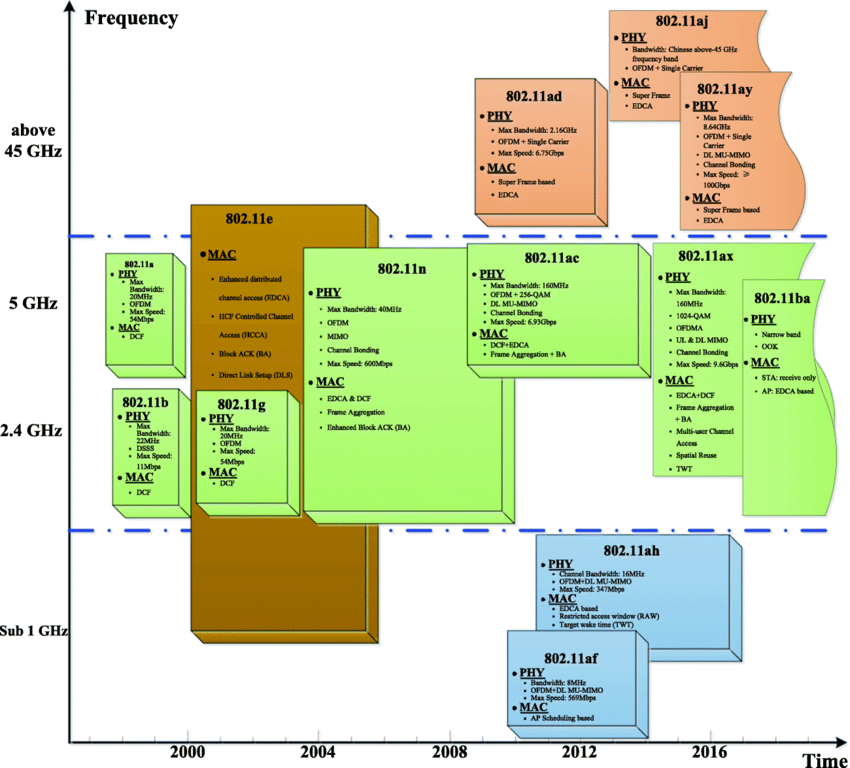
\includegraphics[width=1\textwidth]{evolution.png}
    \caption{Evoluzione dello standard IEEE 802.11}
    \label{fig:evo}
\end{figure}

Un aspetto fondamentale del protocollo IEEE 802.11 è la Distributed Coordination Function (DCF), che rappresenta il metodo standard per l'accesso al canale di comunicazione. DCF è simile al protocollo CSMA/CA (\textit{Carrier Sense Multiple Access with Collision Avoidance}) utilizzato nelle reti cablate quali Ethernet et simila; verrà descritto successivamente.

Non meno importante è l'emendamento IEEE 802.11p (IEEE WAVE), che sarà descritto in modo approfondito successivamente. Questo standard è particolarmente rilevante per le applicazioni di comunicazione veicolare e per la gestione della sicurezza nelle reti di trasporto.

Le caratteristiche tecniche degli standard 802.11 includono l'operatività nelle bande di frequenza a 2.4 GHz e 5 GHz, con l'802.11ax che introduce anche la banda a 6 GHz. Questi standard utilizzano diverse tecniche di modulazione, come BPSK, QPSK e 16-QAM, per ottimizzare la trasmissione dei dati. La larghezza di banda varia: mentre gli standard precedenti utilizzavano larghezze di banda di 20 MHz e 40 MHz, gli standard più recenti come 802.11ac e 802.11ax possono utilizzare larghezze di banda fino a 160 MHz. La tecnologia MIMO consente l'uso di più antenne per trasmettere e ricevere dati simultaneamente, migliorando la capacità e la velocità della rete, mentre il beamforming ottimizza la direzione del segnale verso il dispositivo ricevente, migliorando la portata e l'affidabilità della connessione.

Per quanto riguarda la sicurezza, gli standard 802.11 hanno evoluto i protocolli di protezione nel tempo. Il primo protocollo, WEP (Wired Equivalent Privacy), si è rivelato vulnerabile a vari attacchi, portando all'introduzione di WPA (Wi-Fi Protected Access), che offriva una maggiore sicurezza. Successivamente, WPA2, basato su AES (Advanced Encryption Standard), ha fornito una protezione robusta, mentre WPA3, l'ultima evoluzione, migliora ulteriormente la sicurezza, specialmente in ambienti pubblici e per dispositivi IoT.

\subsection[DCF]{Distributed Coordination Function}
La Distributed Coordination Function (DCF) è la modalità standard attraverso cui i dispositivi Wi-Fi accedono al canale di comunicazione, simile al protocollo CSMA/CA (\textit{Carrier-sense multiple access with collision avoidance}) utilizzato nelle reti cablate, tipo Ethernet et simila. Quando un nodo inizia a trasmettere dati, gli altri dispositivi devono attendere che il canale diventi libero prima di poter inviare le proprie informazioni (\textit{Carrier-sense}).

Dopo che una stazione ha completato la trasmissione dei dati, c'è un intervallo chiamato Short Interframe Space (SIFS), durante il quale l'access point (AP) attende prima di inviare un pacchetto di conferma (ACK). Una volta ricevuto l'ACK, la seconda stazione deve attendere il Distributed Interframe Space (DIFS), che è un periodo di tempo definito per consentire a più nodi di accedere al canale (\textit{Collision Avoidance} - Figura \ref{fig:dcf}). È fondamentale che SIFS sia minore di DIFS, poiché ciò consente ai nodi di tentare di trasmettere i dati, sebbene non necessariamente di farlo immediatamente.

\begin{figure}[h!]
    \centering
    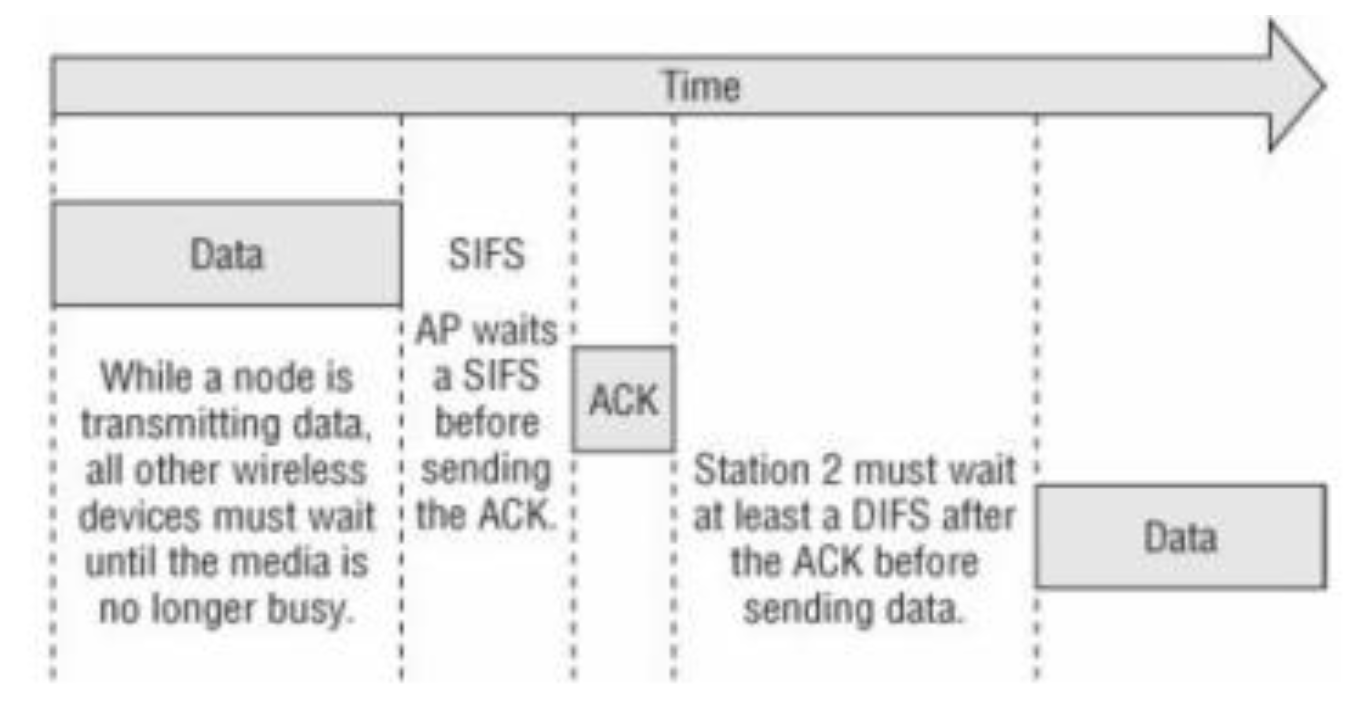
\includegraphics[width=0.7\textwidth]{dcf.png}
    \caption{Distributed Coordination Function}
    \label{fig:dcf}
\end{figure}

Se il canale risulta ancora occupato, il nodo non può semplicemente attendere il DIFS; deve considerare un ulteriore intervallo di backoff per evitare conflitti. Il backoff è un valore casuale scelto all'interno di un intervallo definito da [0, CW], dove CW rappresenta la congestion window, e il suo valore può variare a seconda della situazione della rete. Minore è il valore di CW, minore sarà l'intervallo di attesa. Durante il periodo di contesa, il canale rimarrà inattivo per uno slot temporale, consentendo di decrementare il valore di CW e ridurre l'intervallo di attesa, specialmente in caso di congestione.

Sebbene DCF sia un meccanismo efficace per la condivisione del canale tra più stazioni, presenta alcune limitazioni significative. Innanzitutto, non esiste un controllo della congestione, il che può portare a collisioni. Le collisioni multiple possono limitare la banda disponibile e causare seri problemi di trasmissione. Inoltre, DCF non garantisce alcuna Quality of Service (QoS), non essendoci un metodo per prioritizzare i flussi di traffico.

Per affrontare queste problematiche, esiste un'altra soluzione chiamata Point Coordination Function (PCF), che può essere utilizzata solo in configurazioni infrastrutturate, dove la connessione è gestita da un access point e include meccanismi per garantire la QoS. Tuttavia, poiché PCF non è adatta per il protocollo 802.11p, è necessario integrare la QoS direttamente nella Coordination Function (CF) per garantire prestazioni adeguate nelle reti che non possono utilizzare PCF. Tale problema è stato affrontato con lo sviluppo della EDCA con la \textit{EDCF (Enhanced Distributed Coordination Function)}, affrontata nella \autoref{edca}.

\section{IEEE WAVE}
WAVE è progettato specificamente per ambienti di trasporto, consentendo la comunicazione tra veicoli (\textit{V2V: Vehicle-to-Vehicle}) e tra veicoli e infrastrutture stradali (\textit{V2I: Vehicle-to-Infrastructure}). Questo protocollo sfrutta canali wireless dedicati per garantire una bassa latenza e una maggiore affidabilità, elementi essenziali per applicazioni critiche come la prevenzione degli incidenti e la gestione del traffico. 

Per facilitare questo, l'IEEE ha introdotto un emendamento specifico al protocollo 802.11, noto come 802.11p \cite{std2007wireless}. Questo emendamento si occupa sia del livello fisico, chiamato PHY, sia della gestione dell'accesso al canale, che riguarda il livello MAC. Non ci soffermeremo ulteriormente sui livelli superiori, se non attraverso un breve excursus, poiché il protocollo in questione supporta senza difficoltà qualsiasi tipo di livello, sia esso basato su IP o meno \cite{DSRC-Based-vehicular}. Degno di nota è il fatto che è stato previsto un apposito protocollo per l'invio di frame che non richiedono un livello di trasporto come TCP o UDP, denominato \textit{WAVE Short Message Protocol (WSMP)}.

\begin{figure}[h!]
    \centering
    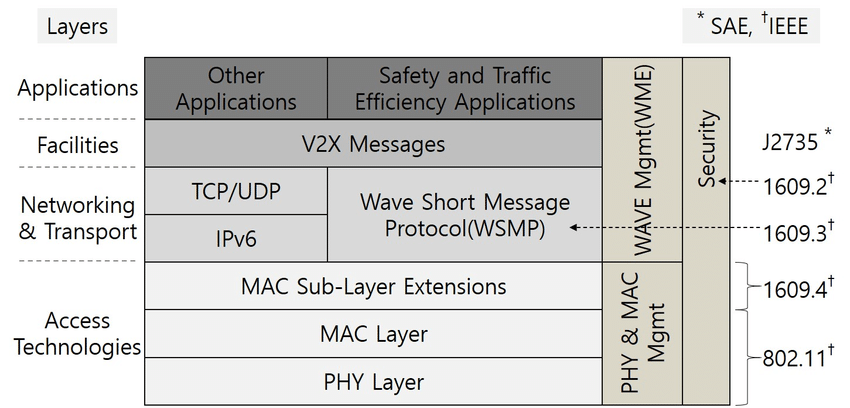
\includegraphics[width=0.7\textwidth]{WAVE-protocol-stack.png}
    \caption{Stack protocollo WAVE}
    \label{fig:wave_stack}
\end{figure}

Di seguito, presentiamo un elenco che fornisce ulteriori dettagli sui protocolli menzionati nella Figura \ref{fig:wave_stack}, partendo dal layer fisico e salendo di volta in volta:

\begin{itemize}
    \item \textit{IEEE 802.11-2016, IEEE Std 802.11p: Wireless Access in Vehicular Environments}.
    \item \textit{IEEE 1609.0: IEEE Guide for Wireless Access in Vehicular Environments (WAVE) Architecture}, con le sue varie  \cite{8686445}: 
        \begin{itemize}
            \item \textit{IEEE 1609.4: IEEE Standard for Wireless Access in Vehicular Environments (WAVE) - Multi-Channel Operation}; per il \textit{channel routing} e il \textit{channel coordination} \cite{7435228}.
            \item \textit{IEEE 1609.3: IEEE Standard for Wireless Access in Vehicular Environments (WAVE) - Networking Services}; per i sopracitati \textit{WAVE Short Messages} \cite{9374154}.
            \item \textit{IEEE 1609.2: IEEE Standard for Wireless Access in Vehicular Environments - Security Services for Applications and Management Messages}; per tutti gli aspetti relativi alla sicurezza \cite{10075082}.
        \end{itemize}
\end{itemize}

Risultano, anche, essere presenti altre varie componenti del protocollo \textit{IEEE 1609.0} su cui non ci si soffermerà e si riportano per completezza:

\begin{itemize}
    \item \textit{IEEE 1609.11:  IEEE Standard for Wireless Access in Vehicular Environments (WAVE) - Over-the-Air Electronic Payment Data}; standard per i pagamenti elettronici in applicazione \textit{WAVE based} \cite{5692959}.
    \item \textit{IEEE 1609.12:  IEEE Standard for Wireless Access in Vehicular Environments (WAVE) - Identifier Allocations}; standard per l'allocazione degli identificatori \textit{WAVE} \cite{8877516}.
\end{itemize}

Per concludere, alla luce del fatto che il contesto preso in esame, quello veicolare, richiede uno scambio di informazioni con latenze minime, \textit{WAVE} si basa interamente su una nuova modalità Wireless, simile alla classica \textit{ad hoc}, chiamata \textit{OCB (Outside Context of a Basic Service Set)}. Questo è un approccio che consente la trasmissione di dati al di fuori delle limitazioni tradizionali delle reti Wi-Fi, permettendo una comunicazione più flessibile e diretta tra i dispositivi, senza la necessità di passare attraverso infrastrutture quali i punti di accesso (\textit{Access Point}).

\subsection[Layer fisico]{Layer fisico}
L'IEEE 802.11p è uno standard della famiglia IEEE 802.11 progettato specificamente per la comunicazione wireless in ambienti vehicolari. È una tecnologia di rete che consente la comunicazione tra veicoli e tra veicoli e infrastrutture, facilitando applicazioni come la sicurezza stradale, la gestione del traffico e i servizi di infotainment.

Esso, innanzitutto, è basato su una modulazione OFDM (\textit{Orthogonal Frequencies Division Multiplexing}), ove in un totale di 64 sottoportanti, ne vengono utilizzate solo 52: 48 per la trasmissione delle informazioni e 4 di tipo pilota (Figura \ref{fig:ofdm}); supporta velocità differenti in base alla modulazione delle sottoportanti e alla larghezza di banda utilizzati.

\begin{figure}[h!]
    \centering
    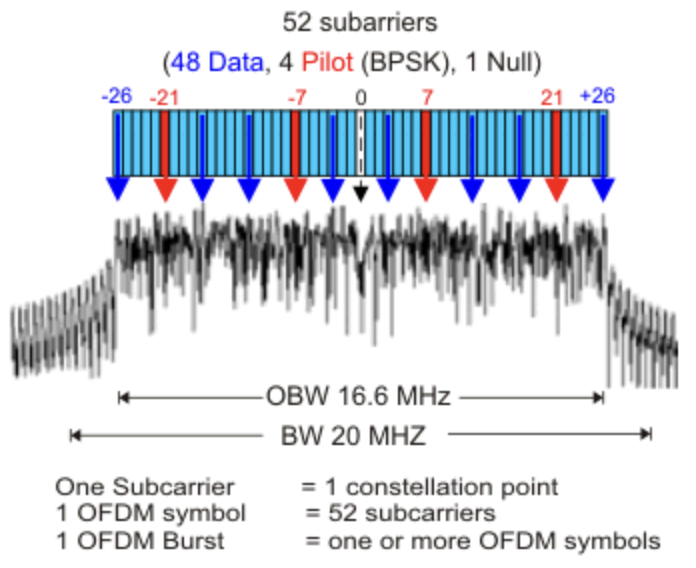
\includegraphics[width=0.4\textwidth]{ofdm.png}
    \caption{OFDM 802.11}
    \label{fig:ofdm}
\end{figure}

Di seguito una tabella riassuntiva dei parametri appena citati, suddivisi per \textit{bandwidth}:

%\clearpage % Forza la stampa delle tabelle e figure in sospeso

\begin{table}[htbp]
    \centering
    \begin{tabular}{|p{7em}|p{7em}|p{7em}|p{7em}|} 
     \hline
     \textbf{Parametri} & \textbf{20 MHz} & \textbf{10 MHz} & \textbf{5 MHz} \\ 
     \hline
     \textbf{Bit rate (Mbit/s)} & 6, 9, 12, 18, 24, 36, 48, 54 & 3, 4.5, 6, 9, 12, 18, 24, 27 & 1.5, 2.25, 3, 4.5, 6, 9, 12, 13.5 \\ 
     \hline
     \textbf{Modulation} & BPSK, QPSK, 16/64QAM & BPSK, QPSK, 16/64QAM & BPSK, QPSK, 16/64QAM \\
     \hline
     \textbf{Code rate} & 1/2, 2/3, 3/4 & 1/2, 2/3, 3/4 & 1/2, 2/3, 3/4 \\
     \hline
     \textbf{Subcarriers} & 52 & 52 & 52 \\
     \hline
     \textbf{Spacing} & 312.5 kHz & 156.25 kHz & 78.125 kHz \\ 
     \hline
    \end{tabular}
    \caption{Parametri delle diverse larghezze di banda}
    \label{table:1}
\end{table}

Parlando circa le frequenze utilizzate, l'IEEE 802.11p opera nella banda di frequenza di 5,9 GHz (5,850 - 5,925 GHz), con le larghezze di canale citate nella Tabella \ref{table:1}. Questo standard consente l'uso di circa 9 canali, come illustrato nella Figura \ref{fig:frequency}. Tra questi, i canali 172 (5.860 GHz) e 184 (5.920 GHz) sono dedicati alla sicurezza: il primo fornisce una soluzione robusta per la sicurezza, mentre il secondo funge da protezione contro la congestione su altri canali \cite{ad_hoc_new}.

\begin{figure}[h!]
    \centering
    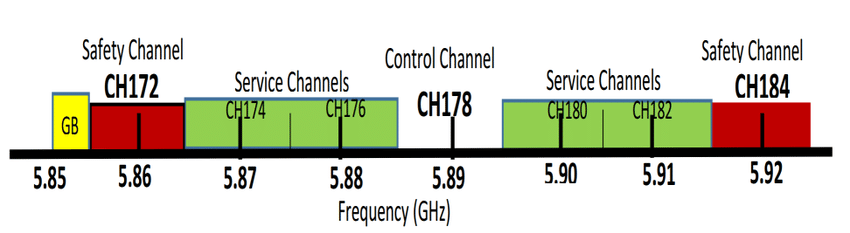
\includegraphics[width=0.7\textwidth]{frequency.png}
    \caption{Frequenze dell'IEEE 802.11p}
    \label{fig:frequency}
\end{figure}

Il canale 178 (5.890 GHz) è un canale di controllo, responsabile della gestione della trasmissione e della creazione del collegamento. Inoltre, sono disponibili sei canali di servizio per la comunicazione bidirezionale tra diversi tipi di unità.

\subsection[Layer MAC]{Layer MAC}
Non esiste una netta distinzione tra il layer MAC dell'IEEE 802.11p con il relativo omonimo del classico IEEE 802.11, se non per alcuni concetti:

\begin{itemize}
    \item come già esplicitato quando si è iniziato a parlare di \textit{WAVE} poc'anzi, esso si basa principalmente sulla modalità \textit{OCB} anzichè le classiche, come ad esempio la \textit{Infrastructure mode}.
    \item per l'accesso al canale, sfrutta una variante della \textit{DCF (Distributed Coordination Function)} chiamata \textit{EDCA (Enhanced Distributed Channel Access)}, sviluppata appositamente per supportare politiche di QoS. A breve verrà affrontato questa nuova \textit{feature} maggiormente nel dettaglio.
\end{itemize}

\subsection[EDCA]{EDCA}
\label{edca}
Nell'EDCA, la differenziazione del servizio è garantita attraverso l'assegnazione di diversi parametri di contesa a ciascuna \textit{Access Category (AC)}. Una stazione QoS può supportare fino a otto priorità utente, che vengono mappate su quattro AC. Ogni AC compete per l'accesso al canale utilizzando impostazioni diverse di AIFS (\textit{Arbitration Inter-frame Space}) e CW (\textit{Contention Window}) \cite{4024121}; per completezza, si riporta nuovamente che l'AIFS determina quanto tempo ogni stazione deve attendere prima di poter iniziare a trasmettere, mentre la CW quanto tempo ciascuna stazione deve aspettare in modo casuale prima di tentare di trasmettere.

A differenza della DCF, dove il DIFS (\textit{Distributed Inter-frame Space}) è utilizzato come IFS (\textit{Inter Frame Space}) comune per consentire a una stazione di accedere al canale, l'EDCF (\textit{Enhanced Distributed Channel Function}) adotta AIFS distinti per ciascuna AC al fine di ottenere una differenziazione nell'accesso. L'AIFS per una specifica AC è definito come segue:

\[AIFS[AC] = AIFSN[AC] * \sigma + SIFS\]

\noindent dove
\begin{itemize}
    \item \textit{AIFSN[AC]} denota un numero per differenziare le AIFS per ogni AC diversa (vedi Tabella \ref{table:2});
    \item \textit{\textsigma} \textit{(slot time)} è un intervallo di tempo dipendente dal layer fisico;
    \item \textit{SIFS (\textit{Short Inter Frame Space})} è il tempo tra un frame di dati e uno di ACK.
\end{itemize}

Questi parametri variano in base a determinate caratteristiche della connessione, come la modulazione utilizzata e l'adozione di tecniche MIMO (Tabella \ref{table:2}).
\begin{table}[h!]
    \centering
    \begin{tabular}{|>{\centering\arraybackslash}p{10em}|>{\centering\arraybackslash}p{7em}|>{\centering\arraybackslash}p{7em}|>{\centering\arraybackslash}p{7em}|} 
     \hline
     \textbf{AC} & \textbf{CWmin} & \textbf{CWmax} & \textbf{AIFSN} \\ 
     \hline
     \textbf{AC\_VO (Voice)} & (aCWmin+1)/4-1 & (aCWmin+1)/2-1 & 2 \\ 
     \hline
     \textbf{AC\_VI (Video)} & (aCWmin+1)/2-1 & aCWmin & 2 \\
     \hline
     \textbf{AC\_BE (Best Effort)} & aCWmin & aCWmax & 7 \\
     \hline
     \textbf{AC\_BK (Background)} & aCWmin & aCWmax & 7 \\
     \hline
    \end{tabular}
    \caption{Parametri delle diverse AC}
    \label{table:2}
\end{table}

Nella Tabella \ref{table:3}, invece, sono riportati i parametri nel caso di aCWmin pari a 31 e aCWmax pari a 1023, come usati, per esempio, nel caso di utilizzo di OFDM e MIMO (\textit{IEEE 802.11n}).
\begin{table}[h!]
    \centering
    \begin{tabular}{|>{\centering\arraybackslash}p{10em}|>{\centering\arraybackslash}p{7em}|>{\centering\arraybackslash}p{7em}|>{\centering\arraybackslash}p{7em}|} 
     \hline
     \textbf{AC} & \textbf{CWmin} & \textbf{CWmax} & \textbf{AIFSN} \\ 
     \hline
     \textbf{AC\_VO (Voice)} & 7 & 15 & 2 \\ 
     \hline
     \textbf{AC\_VI (Video)} & 15 & 31 & 2 \\
     \hline
     \textbf{AC\_BE (Best Effort)} & 31 & 1023 & 7 \\
     \hline
     \textbf{AC\_BK (Background)} & 31 & 1023 & 7 \\
     \hline
    \end{tabular}
    \caption{Parametri delle diverse AC}
    \label{table:3}
\end{table}

E' banale notare che la categoria ad accesso prioritario sarà \textit{AC\_V0}, con la priorità che andrà a scendere siano a \textit{AC\_BK}.

Per comprendere la differenziazione del servizio introdotta da AIFS e CW, possiamo considerare l'esempio mostrato nella Figura \ref{fig:aifs}, in cui sono presenti due stazioni, ciascuna con pacchetti in AC1 e AC4. La differenza di AIFSN (AIFS Number) è di 5, il che significa che l'AC1 della STA1 (Stazione 1) ridurrà il suo contatore di backoff 5 slot prima dell'AC4 della STA2 (Stazione 2). Inoltre, durante questo intervallo, il contatore di backoff dell'AC ad alta priorità può arrivare a zero, consentendo la trasmissione del pacchetto. Questo porta all'occupazione del canale a causa della trasmissione del pacchetto ad alta priorità e alla successiva risincronizzazione.

\begin{figure}[h!]
    \centering
    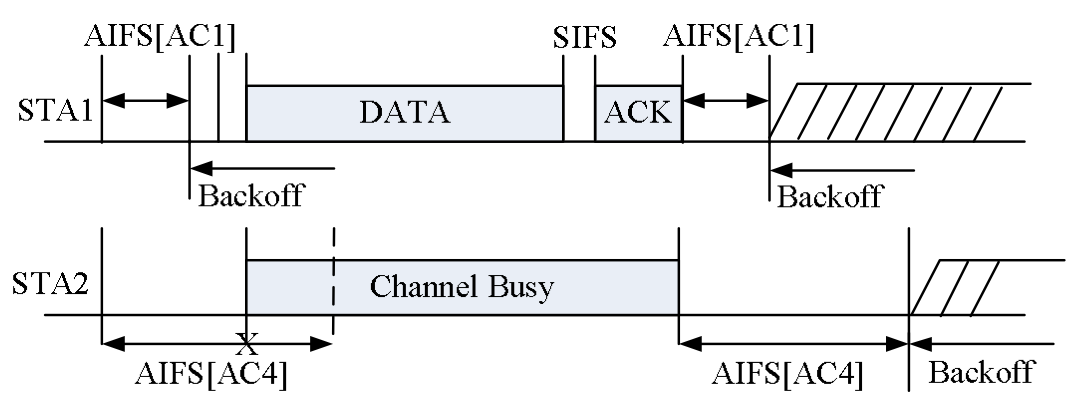
\includegraphics[width=0.7\textwidth]{aifs.png}
    \caption{Accesso al canale nell'EDCA}
    \label{fig:aifs}
\end{figure}

Ad ogni differente AC viene assegnata una differente coda; i vari frame vengono accodati nella coda appropriata in base alla \textit{Class Of Service (CoS)} di appartenenza; quest'ultime risultano essere quelle definite in un altro standard, ovvero l'IEEE 802.1D \cite{1309630}. Il mapping tra classe del frame e AC viene effettuata in questo modo (Tabella \ref{table:4}):

\begin{table}[h!]
    \centering
    \begin{tabular}{|>{\centering\arraybackslash}p{10em}|>{\centering\arraybackslash}p{7em}|} 
     \hline
     \textbf{AC} & \textbf{User Priorities} \\ 
     \hline
     \textbf{AC\_VO (Voice)} & 6, 7 \\ 
     \hline
     \textbf{AC\_VI (Video)} & 4, 5 \\
     \hline
     \textbf{AC\_BE (Best Effort)} & 0, 3 \\
     \hline
     \textbf{AC\_BK (Background)} & 1, 2 \\
     \hline
    \end{tabular}
    \caption{Mappature delle AC con le \textit{User Priorities}}
    \label{table:4}
\end{table}

E', comunque, sempre presente una sorta di casualità tra un AIFSN e un altro in modo da evitare che frame messi nella coda con priorità maggiore monopolizzino il canale a discapito di quelli a priorità minore.

\section[DCC]{Decentralized Congestion Control}
Le comunicazioni C-ITS devono funzionare anche in condizioni di traffico stradale intenso. Se tutti i veicoli partecipano allo scambio di informazioni C-ITS trasmettendo messaggi periodici, è probabile che si verifichi congestione nel canale wireless. Per evitare il degrado delle prestazioni del sistema causato da un carico eccessivo del canale e garantire un accesso equo alle risorse tra le stazioni ITS-G5 vicine (ITS-S), è necessario implementare meccanismi di controllo della congestione. A tal fine, l'ETSI ha pubblicato la specifica \textit{TS 102 687}, che definisce un meccanismo di controllo della congestione decentralizzato (\textit{DCC - Decentralized Congestion Control}) come parte dello stack di protocolli ITS-G5 \cite{8535090}. Il DCC è un componente obbligatorio dell'ITS-S e opera nella banda di frequenza dei 5,9 GHz.

Esso ha introdotto un approccio a macchina a stati finti al livello di accesso per adattare diversi parametri di trasmissione in base al carico del canale misurato. Ogni stato della macchina è associato a un determinato livello di carico del canale e a un insieme specifico di parametri di trasmissione. Questo consente al DCC di ottimizzare le comunicazioni in situazioni di congestione, migliorando l'efficienza e le prestazioni del sistema C-ITS.

Esistono diverse configurazioni che prevedono molteplici stati nella macchina di stato, ma ci concentreremo in particolare sulla configurazione \textit{DCC 2+1}, che comprende tre stati distinti: \textit{Relaxed}, \textit{Active} e \textit{Restrictive} (Figura \ref{fig:dcc}).

\begin{figure}[h!]
    \centering
    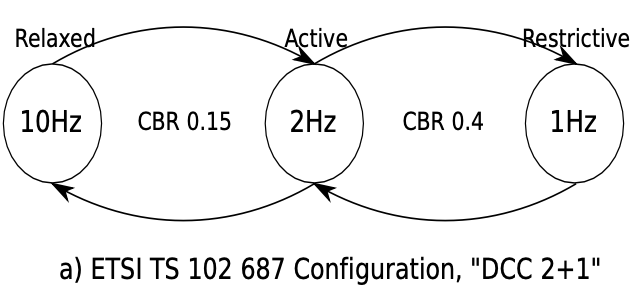
\includegraphics[width=0.7\textwidth]{dcc.png}
    \caption{DCC nella configurazione \textit{"2+1"}}
    \label{fig:dcc}
\end{figure}

In ciascuno stato del DCC vengono definite restrizioni sui parametri di trasmissione. L'ETSI DCC considera in generale cinque meccanismi per controllare l'accesso al canale del veicolo:

\begin{itemize}
    \item \textit{Transmit Power Control (TPC)} che adatta la potenza di trasmissione;
    \item \textit{Transmit Rate Control (TRC)} che adatta l'intervallo di trasmissione dei pacchetti;
    \item \textit{Transmit Datarate Control (TDC)} che adatta il \textit{data rate};
    \item \textit{DCC Sensitivity Control (DSC)} che adatta dinamicamente il \textit{CCA Sensitivity Threshold (CSThresh)}, ovvero la soglia sotto la quale il canale viene rilevato libero e non occupato;
    \item \textit{Transmit Access Control (TAC)} che apre e chiude dinamicamente l'accesso dei pacchetti con una determinata priorità alla relativa coda di trasmissione.
\end{itemize}

\noindent Maggiori dettagli su tali parametri verranno forniti nella \autoref{parametri_dcc}.

La scelta dello stato DCC si basa sulla valutazione del Channel Busy Ratio (CBR). L'ETSI propone un metodo di riferimento per stimare il valore del CBR consistente nel campionare tale valore ad intervalli prefissati per la durata di 1 secondo (Figura \ref{fig:cbr}); tale modello può, tuttavia, cambiare in base all'hardware utilizzato e al contesto di utilizzo.

\begin{figure}[h!]
    \centering
    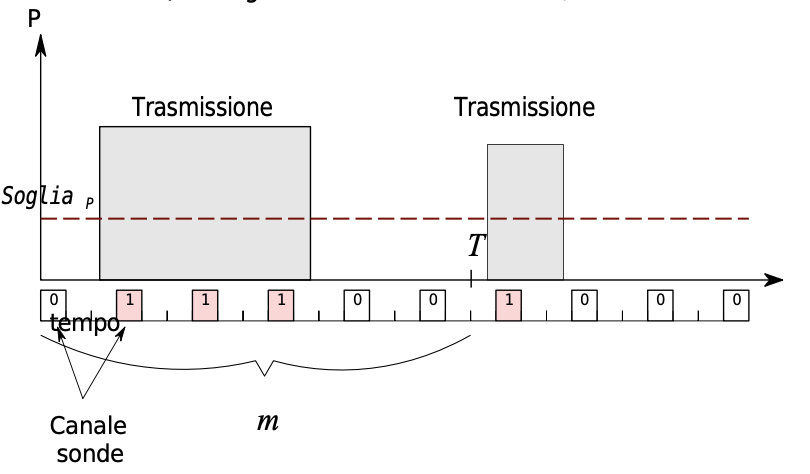
\includegraphics[width=0.7\textwidth]{cbr.png}
    \caption{Misurazione del CBR}
    \label{fig:cbr}
\end{figure}

Ogni transizione nella macchina a stati ha un valore CBR corrispondente come soglia (Figura \ref{fig:dcc}); la transizione viene eseguita in
una delle due condizioni seguenti:
\begin{itemize}
    \item \textit{Passaggio a uno stato più restrittivo}: se il valore CBR era superiore alla soglia durante l'ultimo intervallo di misurazione osservato.
    \item \textit{Passaggio a uno stato meno restrittivo}: se il CBR è stato inferiore alla soglia durante gli ultimi cinque intervalli di misurazione consecutivi osservati.
\end{itemize}

\subsection[Parametri DCC]{Parametri DCC}
\label{parametri_dcc}
Vengono mostrati i parametri relativi al DCC con i relativi valori in base allo stato \cite{6686471} (Tabella \ref{table:5}).

TPC (Transmit Power Control), DSC (DCC Sensitivity Control) e TRC (Transmit Rate Control) sono stati scelti per l'analisi perché sono direttamente rilevanti per le applicazioni di sicurezza cooperativa, dove la priorità è garantire comunicazioni affidabili e tempestive. Questi meccanismi si concentrano sull'ottimizzazione della potenza di trasmissione, della sensibilità e del tasso di trasmissione, elementi cruciali per mantenere la qualità del segnale e ridurre i ritardi in situazioni di congestione.

D'altra parte, TDC (Transmit Datarate Control) e TAC (Transmit Access Control) sono stati scartati per motivi specifici. La TDC è meno pertinente perché esiste un consenso consolidato nell'impostare a 6 Mbps la velocità di trasmissione per i messaggi di sicurezza, rendendo superflua la necessità di adattamenti dinamici della velocità. Questo approccio standardizzato garantisce una trasmissione stabile, essenziale in contesti critici.

La TAC, invece, è stata esclusa poiché si occupa principalmente della gestione della priorità tra diversi flussi di traffico, un aspetto meno rilevante per le comunicazioni di sicurezza. In questo contesto, l'obiettivo principale è garantire che i messaggi critici vengano trasmessi senza ritardi, piuttosto che gestire la priorità tra vari tipi di dati. Pertanto, concentrarsi su TPC, DSC e TRC consente di affrontare in modo più efficace le sfide specifiche delle comunicazioni di sicurezza cooperativa.

\begin{table}[h!]
    \centering
    \begin{tabular}{|>{\centering\arraybackslash}p{3em}|>{\centering\arraybackslash}p{5em}|>{\centering\arraybackslash}p{7em}|>{\centering\arraybackslash}p{7em}|>{\centering\arraybackslash}p{7em}|} 
     \hline
     \textbf{Scheme} & \textbf{Metric} & \textbf{RELAXED} & \textbf{ACTIVE} & \textbf{RESTRICTIVE} \\ 
     \hline
     \textbf{TPC} & \textit{\( P_{t} \)} & 35 dBm & 15 dBm & -10 dBm \\ 
     \hline
     \textbf{DSC} & \textit{CSThresh} & -95 dBm & -85 dBm & -65 dBm \\
     \hline
     \textbf{TRC} & Pack. inter. & 0.04 s & 0.5 s & 1 s\\
     \hline
    \end{tabular}
    \caption{Parametri DCC}
    \label{table:5}
\end{table}

Degno di nota il fatto che, nonostante i validi obiettivi delle tecniche DCC specificate dall'ETSI, finora solo pochi studi hanno analizzato le loro prestazioni. Ci sono solo alcuni lavori, come quello di Subramanian et al. \cite{subramanian2012congestion}, ove tutti i meccanismi DCC sono stati attivati in modo simulato, e i risultati indicano che non sono efficaci nel controllare la congestione e garantire la raggiungibilità. Gli autori propongono quindi miglioramenti alla tecnica TPC, progettando una macchina a stati con sei stati e una soglia di carico del canale più alta per lo stato di congestione. Tuttavia, entrambi i lavori non distinguono gli effetti di ciascun meccanismo.

\subsection[DCC con code EDCA]{Parametri DCC con code EDCA}

In aggiunta alle tecniche di controllo della congestione già specificate, l'ETSI ha introdotto parametri aggiuntivi in base alle categorie di accesso (Access Categories, AC) utilizzate \cite{etsi2011intelligent} (Figura \ref{fig:dcc_edca}). Queste categorie sono fondamentali per gestire le diverse priorità e requisiti di latenza delle comunicazioni veicolari. Ogni Access Category è associata a specifiche caratteristiche di traffico, consentendo una gestione più fine delle risorse di comunicazione.

Ad esempio, le applicazioni critiche per la sicurezza, come i messaggi di avviso e le comunicazioni di emergenza, possono essere classificate in una categoria di accesso con priorità più alta. Ciò implica l'adozione di parametri di controllo della congestione più stringenti per garantire che questi messaggi vengano trasmessi senza ritardi. Al contrario, le comunicazioni meno critiche possono essere assegnate a categorie con requisiti di latenza e affidabilità inferiori, permettendo una gestione più flessibile delle risorse di rete.

Questa suddivisione in Access Categories consente all'ETSI di ottimizzare le prestazioni del sistema, migliorando l'efficacia delle tecniche di controllo della congestione e garantendo che le comunicazioni più importanti ricevano la priorità necessaria in situazioni di traffico intenso.

\begin{figure}[h!]
    \centering
    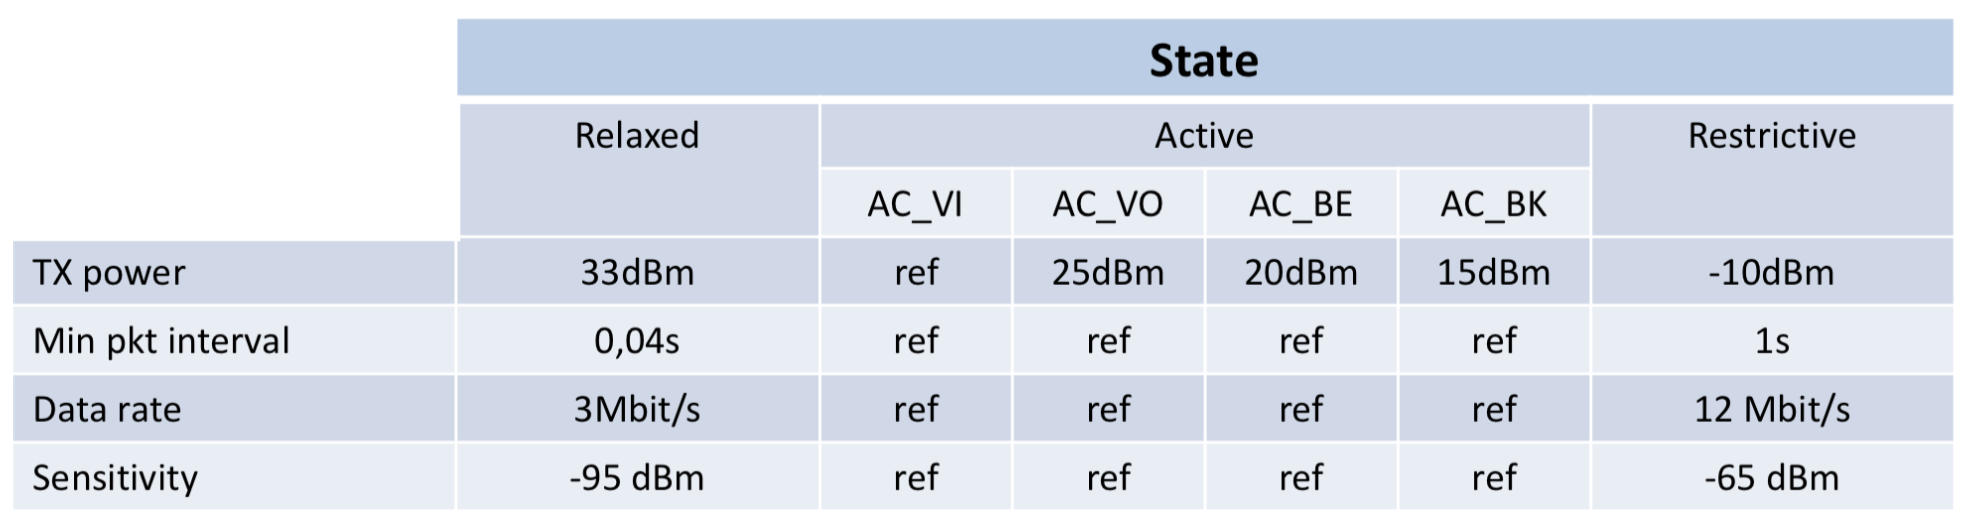
\includegraphics[width=1\textwidth]{dcc_edca.png}
    \caption{Parametri DCC con code EDCA}
    \label{fig:dcc_edca}
\end{figure}

Il valore \textit{ref} indica che il parametro è invariato e viene utilizzato il valore precedente del parametro di riferimento corrispondente.

Da come si può notare in figura \ref{fig:dcc_edca}, in questo contesto non è stata esclusa la \textit{Transmit Datarate Control}, in quanto, vista l'applicazione del DCC con code EDCA in contesti generici e non strettamente legati alla sicurezza, non aveva più senso basarsi sullo standard \textit{de facto} della velocità di trasmissione di 6 Mbps.

\chapter{Testbed}

Per l'implementazione del testbed necessario a eseguire una varietà di test, sono state esaminate numerose schede di sviluppo disponibili sul mercato, caratterizzate da prezzi competitivi e disponibilità immediata. A causa dell'aumento esponenziale dei costi delle varie versioni di Raspberry Pi, soprattutto a seguito della pandemia di Covid-19 e della conseguente scarsità di offerta, si è deciso di escludere a priori queste opzioni.

Inizialmente, si è considerata l'Arduino Yun, una scheda del noto brand Arduino. Tuttavia, si è subito riscontrato che le sue prestazioni erano insufficienti e che gli strumenti forniti non garantivano la flessibilità desiderata. In particolare, la shell risultava poco performante e non era possibile impostare tempi di sleep inferiori a un secondo. Inoltre, è importante notare che l'Arduino Yun è stato deprecato a favore di altre schede, che, sebbene più performanti, non offrivano lo stesso rapporto qualità-prezzo.

Successivamente, si è passati all'analisi di router Mikrotik, ma anche in questo caso le prestazioni e la flessibilità nelle configurazioni non hanno soddisfatto le aspettative.

Alla fine, la soluzione ottimale è stata trovata nelle schede Rock 3 Model A (\ref{fig:testbed}). Queste schede, pur essendo leggermente più economiche rispetto ai Raspberry Pi, offrivano le prestazioni, la flessibilità e il costo contenuto ricercati. Sono state utilizzate quattro unità, tutte configurate in modo identico con Armbian OS come sistema operativo. Ulteriori dettagli verranno forniti in seguito.

\begin{figure}[h!]
    \centering
    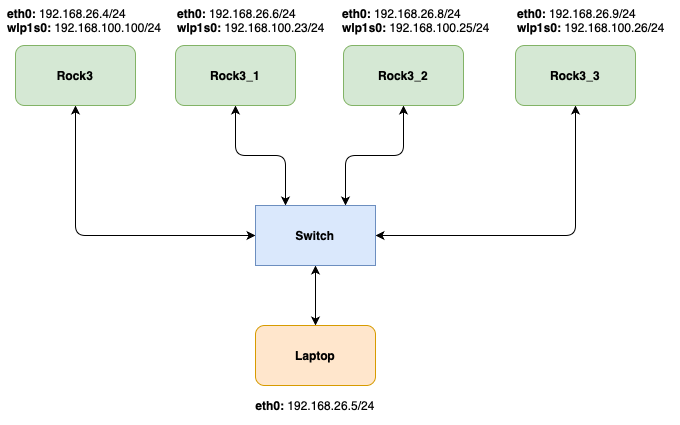
\includegraphics[width=0.7\textwidth]{testbed_cambia.png}
    \caption{Testbed}
    \label{fig:testbed}
\end{figure}

Per l'esecuzione delle varie prove, sono stati utilizzati due software: iPerf 2 e Netcat versione OpenBSD.

\section{Rock 3 Model A board}

Il Rock 3 Model A è una scheda di sviluppo avanzata, progettata per applicazioni che richiedono elevate prestazioni di calcolo, rendendola particolarmente adatta per progetti di Internet of Things (IoT), edge computing e server leggeri. 

Al centro di questa scheda si trova il processore Rockchip RK3566, un potente quad-core ARM Cortex-A55 che può raggiungere una frequenza di clock fino a 2.0 GHz. Questa architettura a 64 bit consente di gestire una vasta gamma di applicazioni moderne in modo efficiente. La scheda è dotata di 2 GB di RAM LPDDR4, che garantiscono prestazioni elevate e una gestione efficace delle applicazioni multitasking. Per quanto riguarda l'archiviazione, il Rock 3 Model A offre uno slot per schede microSD, permettendo di espandere facilmente la capacità di memoria, oltre a supportare eMMC fino a 64 GB. Per la connettività, è equipaggiata con una porta Gigabit Ethernet, che assicura una connessione di rete ad alta velocità, e diverse porte USB 3.0 e USB 2.0 per il collegamento di dispositivi esterni. 

Sebbene non sia una caratteristica fondamentale per i nostri scopi, è interessante notare che la scheda include anche una GPU Mali-G52, che consente una buona elaborazione grafica, rendendola adatta per applicazioni multimediali e giochi leggeri. Il Rock 3 Model A offre ampie possibilità di espandibilità, grazie ai pin GPIO (General Purpose Input/Output) che consentono di collegare sensori, attuatori e altri dispositivi. Supporta varie interfacce di comunicazione, come I2C, SPI e UART, facilitando l'integrazione con altri componenti hardware. Per quanto riguarda l'alimentazione, la scheda può essere alimentata tramite un connettore DC o tramite USB-C, offrendo flessibilità nelle opzioni di alimentazione.

La compatibilità con diversi sistemi operativi, tra cui varie distribuzioni Linux come Armbian e Android, rende il Rock 3 Model A estremamente versatile per una varietà di progetti; in particolare, nel nostro caso, si è preferito adottare Armbian OS in quanto risulta essere quello più simile ad un classico sistema \textit{Linux-based} ed inoltre, cosa non di poco conto, fornisce una toolchain comprendente una serie di strumenti e componenti necessari per la compilazione e per il debugging.

\subsection[Atheros Wi-Fi card]{Atheros Wi-Fi card}
Il Rock 3 descritto sopra non monta \textit{out-of-the-box} una scheda di rete che fornisce la connettività Wireless (IEEE 802.11), in virtù di ciò si è reso necessario aggiungerne una esterna collegandola mediante l'interfaccia \textit{PCI Express - M.2 Specification} che la board fornisce per permettere l'espansione delle sue funzionalità hardware.

Tra le varie soluzione in commercio, la scelta è ricaduta sull'adattatore Qualcomm Atheros AR9462. Esso supporta gli standard Wi-Fi 802.11a/b/g/n e permette l'utilizzo della modalità OCB (\textit{Outside the Context of BSS}) utilizzata nel nostro caso al fine di permettere la comunicazione senza fili tra i vari dispositivi senza la necessità di stabilire un \textit{Basic Service Set}.

Un altro aspetto fondamentale che ha reso possibile il nostro lavoro è la possibilità di accedere a una vasta gamma di dati e statistiche sul funzionamento dell'interfaccia di rete, abilitando i flag appropriati durante la compilazione del kernel. Queste informazioni, infatti, non sono generalmente disponibili per la maggior parte delle schede di rete commerciali, rendendo la nostra analisi molto più approfondita e dettagliata. E' possibile accedere a tali statistiche mediante il comando \verb|iw wlp1s0 survey dump| oppure andando ad effettuare un dump dei registri interni della scheda con

\begin{lstlisting}
cat /sys/kernel/debug/ieee80211/phy0/ath9k/regdump
\end{lstlisting}

\noindent Non ci soffermeremo su quest'ultima possibilità in quanto esula dal nostro scopo.

Infine, la natura completamente open-source dei suoi driver ha permesso di apportare ad esso le piccole modifiche necessarie al nostro scopo.

\subsection[Connessione con le board]{Connessione con le board}
Le quattro schede utilizzate nel progetto, come descritto prima, sono dotate di due interfacce di rete distinte, ciascuna con un ruolo specifico nel funzionamento complessivo del sistema. La prima interfaccia è una connessione wireless, utilizzata esclusivamente per l'esecuzione dei test.

La seconda interfaccia è una connessione Ethernet, progettata specificamente per consentire un'interazione diretta con le schede, permettendo così l'invio di comandi per la configurazione, l'avvio e la chiusura dei test, tutti gestiti da un PC.

I quattro dispositivi sono stati collegati a uno switch Ethernet a cinque porte, mentre la porta aggiuntiva è stata riservata per la connessione del PC. Nell'immagine \ref{fig:etichetta} è mostrata la topologia di rete con i vari indirizzi IP assegnati.

\begin{figure}[h!]
    \centering
    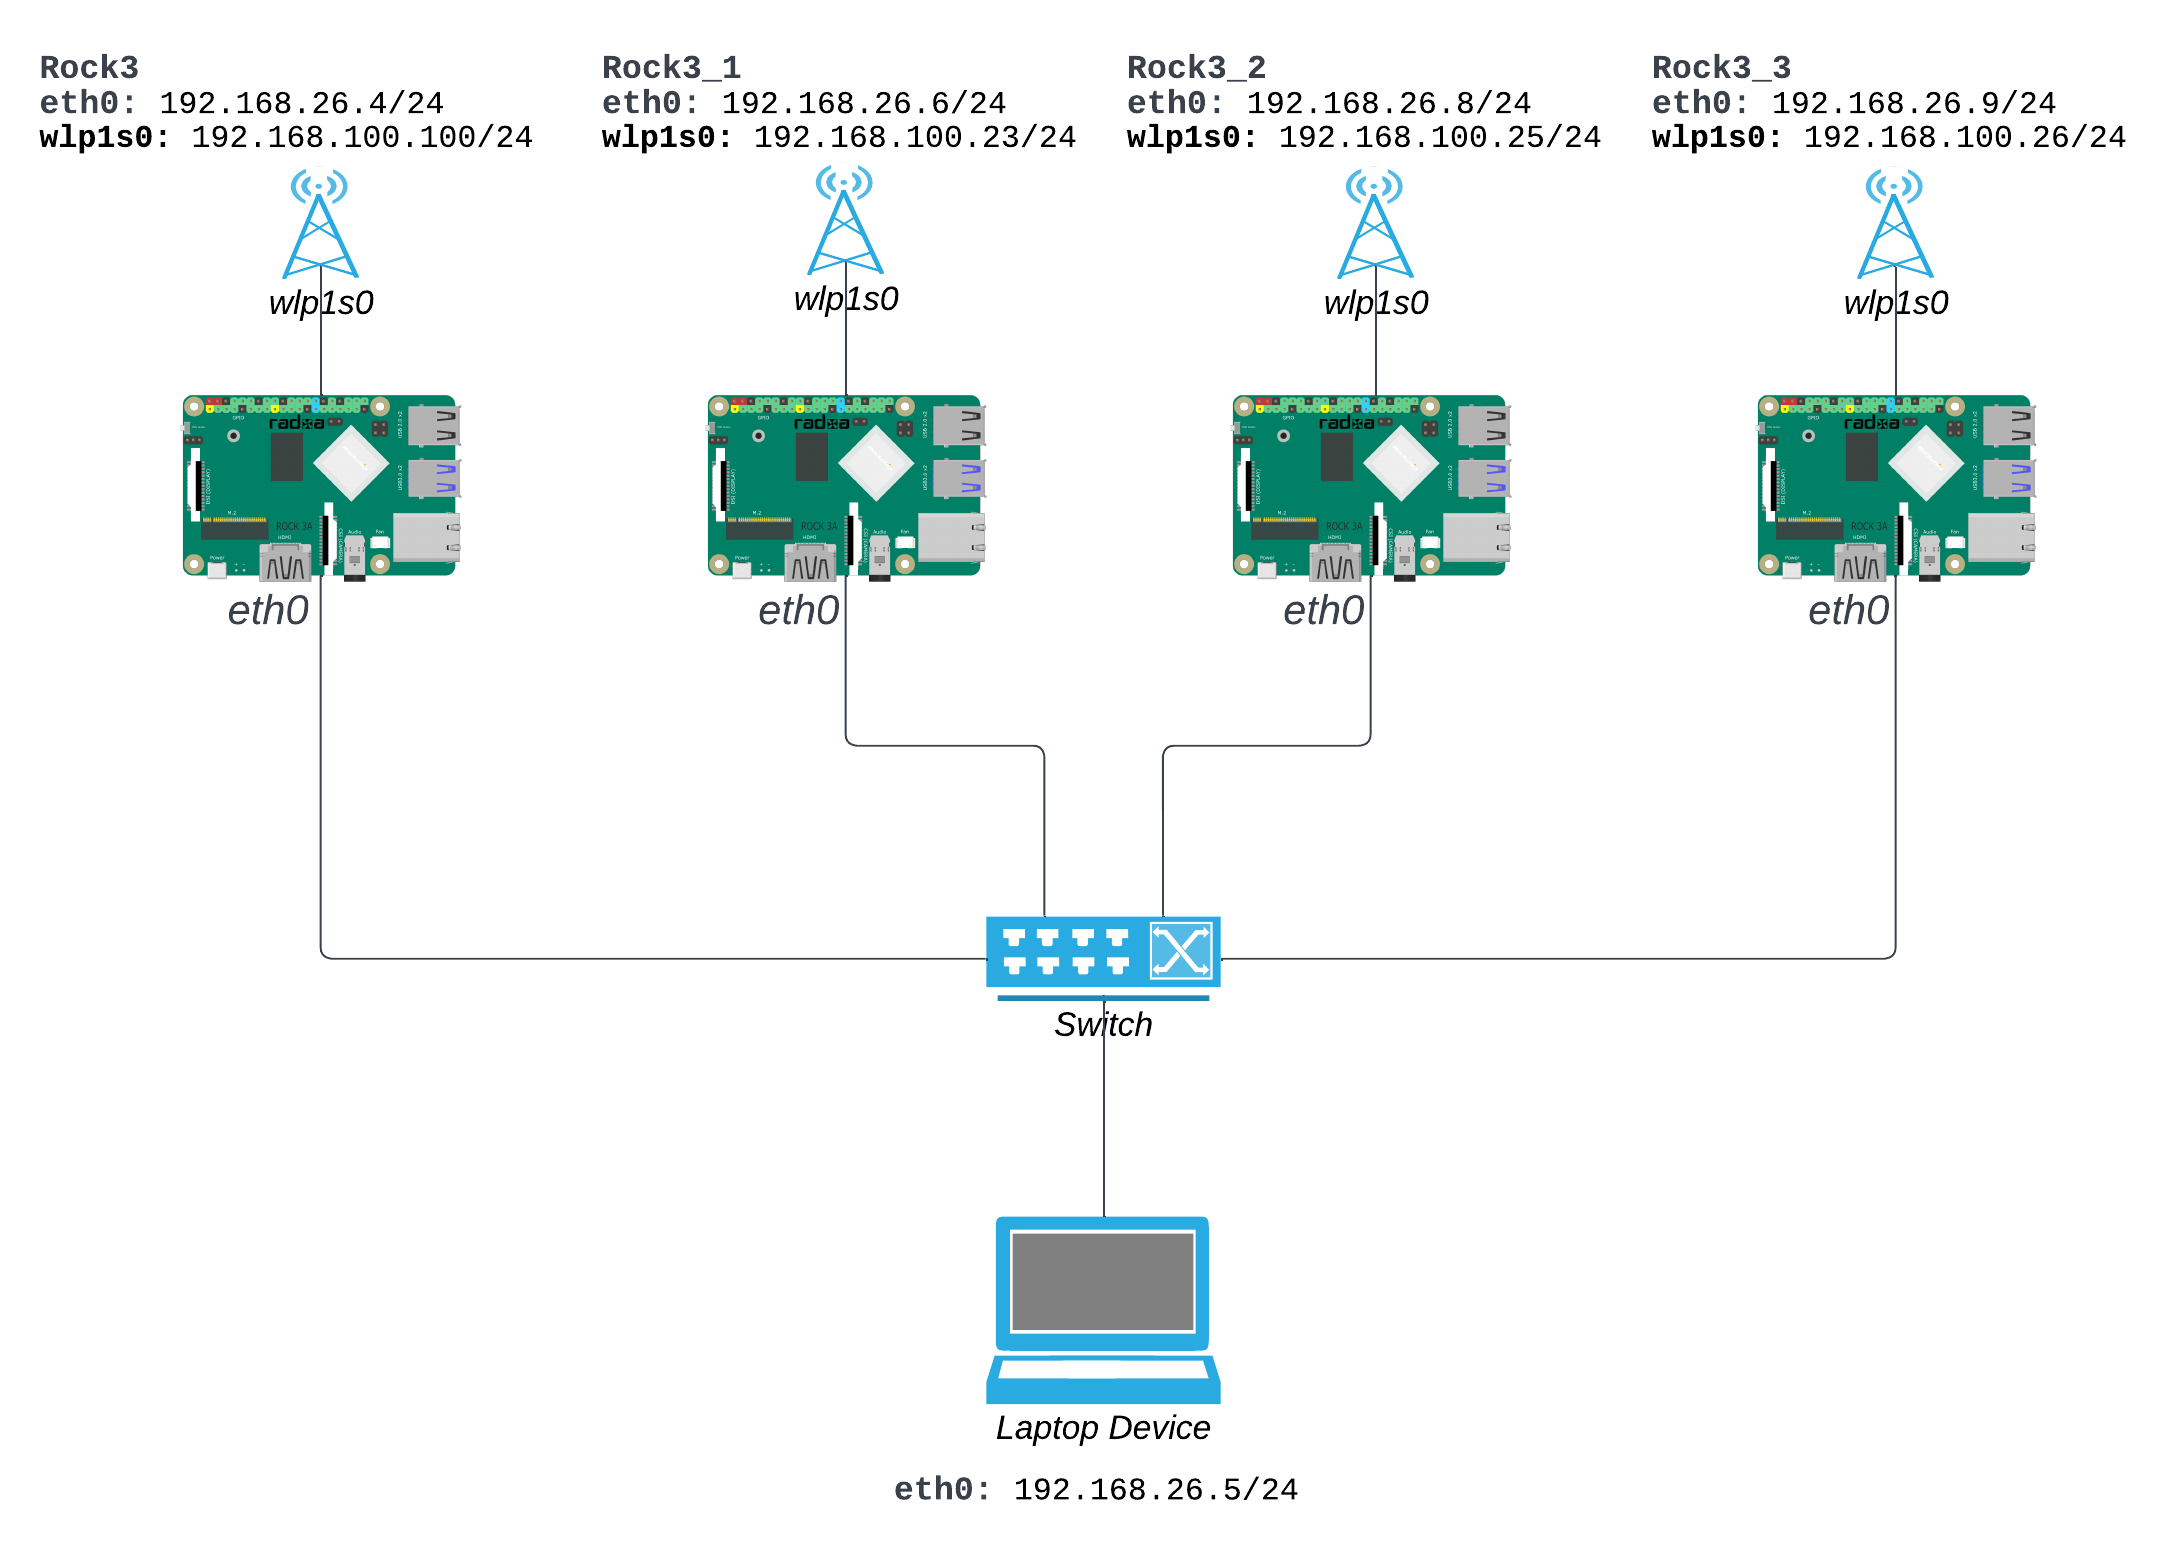
\includegraphics[width=0.7\textwidth]{topology.png}
    \caption{Topologia rete}
    \label{fig:etichetta}
\end{figure}

La connessione avviene mediante il protocollo sicuro SSH, ma non ci si soffermerà su di esso in quanto questo esula dagli obiettivi del presente testo.

\subsection[Impostazione interfaccia Wi-Fi]{Impostazione interfaccia Wi-Fi}
L'interfaccia Wi-Fi di ogni singolo dispositivo Rock, al fine di avere una conessione wireless di tipo OCB funzionante, è stata configurata con i seguenti comandi:

\begin{lstlisting}
    ip link set dev wlp1s0 down
    # imposta la tipologia come ad-hoc
    iw wlp1s0 set type ocb
    # accende l'interfaccia
    ip link set dev wlp1s0 up
    
    iw wlp1s0 ocb join 2462 10MHz
    ip addr add 192.168.100.xxx/24 dev wlp1s0
    ip route add default via 192.168.100.xxx dev wlp1s0
\end{lstlisting}

Non si entrerà nel dettaglio di questi comandi, del resto abbastanza ovvi; ci si limita ad esplicitare che l'interfaccia è stata settata in modalità OCB (\textit{Outside the Context of BSS}), è stato scelto il canale 11, con frequenza fondamentale f\ped{0} pari a 2462 MHz e che, naturalmente, viene assegnato un indirizzo IP con la rispettiva rotta.

\section{Tweaking}
Per rendere possibili alcune configurazioni nei dispositivi Rock e la raccolta dei dati, si è reso necessario mettere mano nalel codice sorgente del Kernel Linux ed applicare alcune patch.

Nella fattispecie, si è dovuto provvedere ad abilitare la \textit{Debug Mode} messa a disposizione dal driver \textit{Ath9k} della scheda di rete wireless ma disabilitata in maniera predefinita, una piccola modifica all'output delle statistiche di rete accessibili dall'utente e l'abilitazione delle code separate per le quattro \textit{Access Categories}.

Tutto ciò è stato reso possibile grazie a patch e a informazioni fornite dalla comunità open source e alla documentazione del produttore.

Viene fornita, inizialmente, una descrizione separata delle varie modifiche apportate, esplicitiando alla fine del trittico il processo di compilazione necessario. Importante notare che le varie patch sono state scritte esclusivamente per la versione del kernel Linux \textit{rockchip64-6.6}, l'ultima disponibile al momento della configurazione del testbed; non si garantisce che possano essere applicate senza ulteriori modifiche ad altre versioni, sia che esse siano sulla architettura ARM che differente.

\subsection[Debug Mode]{Debug Mode}
Per l'abilitazione della suddetta modalità, si è semplicemente messo mano al file \textit{linux-rockchip64-current.config}, file di configurazione utilizzato dalla \textit{toolchain} di compilazione del Kernel del sistema Armbian, abilitando tre differenti flag\cite{linux_wireless}:

\verb|CONFIG_ATH9K_HTC_DEBUGFS=y|

\verb|CONFIG_ATH9K_HWRNG=y|

\verb|CONFIG_ATH9K_DEBUGFS=y|

\subsection[Queues]{Queues}
La patch \textit{00550-ac.patch} fornita modifica un segmento di codice nel file wme.c del driver mac80211, che gestisce la classificazione dei pacchetti in una rete wireless.
Molto semplicemente, si è provveduto ad eliminare la classificazione effettuata dal driver \textit{mac80211} in quanto il suo comportamento andava in conflitto con le Access Categories utilizzate e dirottava tutti i pacchetti sulla coda \textit{Best Effort (BE)}, indipendentemente dalla categoria scelta.
Il problema è dovuto all'introduzione delle cosiddette "code software intermedie" all'interno del driver "mac80211", per i driver supportati\cite{intermediate_queue} come l'\textit{Ath9k}.

\begin{lstlisting}
    --- a/net/mac80211/wme.c        2024-06-17 11:16:29
    +++ b/net/mac80211/wme.c        2024-06-17 11:17:12
    @@ -176,9 +176,9 @@
     
            /* use the data classifier to determine what 802.1d tag the
             * data frame has */
    -       qos_map = rcu_dereference(sdata->qos_map);
    -       skb->priority = cfg80211_classify8021d(skb, qos_map ?
    -                                              &qos_map->qos_map : NULL);
    +       //qos_map = rcu_dereference(sdata->qos_map);
    +       //skb->priority = cfg80211_classify8021d(skb, qos_map ?
    +                                              //&qos_map->qos_map : NULL);
     
      downgrade:
            return ieee80211_downgrade_queue(sdata, sta, skb);
\end{lstlisting}
Questa caratteristica è stata introdotta per spostare l'implementazione delle code più verso il lato software del sottosistema wireless, consentendo all'hardware di mantenere solo code brevi e permettendo anche una maggiore equità tra le stazioni che comunicano.

La possibilità di utilizzare correttamente le categorie di accesso insieme alle code software del \textit{mac80211} risulta essere in fase di implementazione da parte della comunità al momento della stesura di questo elaborato.

\subsection[Statistiche occupazione canale]{Statistiche occupazione canale}
La patch fornita, di nome \textit{00551-ac.patch}, modifica un segmento del codice nel file link.c del driver \textit{ath9k}, che è parte della gestione delle statistiche di monitoraggio della rete wireless. Esso in maniera predefinita restituiva, mediante il comando \verb|iw wlp1s0 survey| \verb|dump|, varie statistiche tra cui i tempi in cui, rispettivamente, il canale risulta essere occupato, viene usato per trasmettere e ricevere da parte dell'interfaccia. 

Questi valori venivano mostrati in output in maniera incrementale, ovvero ogni valore campionato era sommato al valore precedente; tale modus operandi complicava la raccolta dei dati nel nostro caso e si è provveduto a modificare il codice in modo che i valori vengano mostrati, singolarmente, volta per volta.
\begin{lstlisting}
    --- a/drivers/net/wireless/ath/ath9k/link.c	2024-06-21 11:46:11
    +++ b/drivers/net/wireless/ath/ath9k/link.c	2024-06-21 11:47:38
    @@ -524,10 +524,10 @@
                 SURVEY_INFO_TIME_BUSY |
                 SURVEY_INFO_TIME_RX |
                 SURVEY_INFO_TIME_TX;
    -		survey->time += cc->cycles / div;
    -		survey->time_busy += cc->rx_busy / div;
    -		survey->time_rx += cc->rx_frame / div;
    -		survey->time_tx += cc->tx_frame / div;
    +		survey->time = cc->cycles / div;
    +		survey->time_busy = cc->rx_busy / div;
    +		survey->time_rx = cc->rx_frame / div;
    +		survey->time_tx = cc->tx_frame / div;
         }
     
         if (cc->cycles < div)
\end{lstlisting}
Giusto per completezza, viene mostrato l'output dell'esecuzione del comando 

\verb|iw| \verb|wlp1s0 survey dump|:
\begin{lstlisting}
root@rock-3a:~# iw wlp1s0 survey dump
    Survey data from wlp1s0
	frequency:			2462 MHz [in use]
	noise:				-93 dBm
	channel active time:		136546 ms
	channel busy time:		1642 ms
	channel receive time:		1496 ms
	channel transmit time:		0 ms
\end{lstlisting}
Per semplicità viene mostrato qui solo l'output relativo al canale 11, omettendo le informazioni relative agli altri canali.

Per calcolare il carico del canale, ovvero la percentuale di tempo in cui il canale wireless è occupato, sono stati raccolti due valori fondamentali: il \textit{channel active time} e il \textit{channel busy time}. Il primo rappresenta il tempo in cui l'interfaccia è attiva per trasmettere, ricevere o ascoltare il canale, mentre il secondo indica il tempo in cui l'interfaccia è attiva ma in attesa a causa dell'occupazione del canale\cite{han2016adaptive}.
\subsection[Kernel building]{Kernel building}
Per la compilazione dell'intero sistema Armbian o, nello specifico, del Kernel, ci si è basati sulla toolchain messaci a disposizione dalla comunità open source. 

La toolchain di Armbian è una componente essenziale per sviluppare e ottimizzare software per dispositivi ARM, specialmente quando si lavora con macchine host x86. Il cuore di questa toolchain è il compilatore GCC, configurato specificamente per il target ARM. Questo compilatore traduce il codice sorgente in codice eseguibile ottimizzato per le architetture ARM, permettendo di sfruttare appieno le capacità hardware dei dispositivi.

Un suo aspetto cruciale è la cross-compilazione. Lavorare con dispositivi ARM spesso significa confrontarsi con limitazioni di risorse hardware che rendono impraticabile la compilazione diretta. La cross-compilazione risolve questo problema permettendo di compilare il software su una macchina più potente (solitamente un PC x86) e poi eseguirlo sul dispositivo ARM. Questo processo non solo accelera notevolmente la compilazione, ma evita anche il rischio di esaurire le risorse durante la build.

Il sistema di build automatizzato di Armbian gioca un ruolo centrale nella gestione di questo processo. Gli script e gli strumenti inclusi orchestrano la compilazione del kernel, del bootloader e dei vari pacchetti software, assicurando che tutto sia perfettamente integrato e ottimizzato. Questo sistema è pensato per gestire le complessità della cross-compilazione, semplificando il processo per gli sviluppatori.

Non ci si dilungherà nelle modalità di download e installazione di tutto il pacchetto, in quanto è tranquillamente reperibile in rete e richiede, per la sua configurazione iniziale, componenti esterne quali Docker. Una volta installato e funzionante, fatte le modifiche ad-hoc al file di configurazione (il citato precedentemente file \textit{linux-rockchip64-current.config}) ed inserite le patch già menzionate nella cartella

\verb|~/build/patch/kernel/archive/rockchip64-6.6 |

\noindent e si procede alla compilazione mediante il comando 

\verb|./compile.sh kernel ARTIFACT_IGNORE_CACHE='yes' \| 

\verb|BOARD=rock-3a BRANCH=current|

\noindent Il processo restituirà il nuovo kernel pacchettizzato all'interno di file \textit{.deb}, che andranno installati sui dispositivi come di consueto.

\section{iPerf con Access Categories abilitate}
iPerf è un software di benchmarking di rete utilizzato per misurare le prestazioni della larghezza di banda e della latenza nelle connessioni TCP e UDP. Permette di misurare la larghezza di banda disponibile tra due punti di rete, offrendo la possibilità di testare sia il protocollo TCP, orientato alla connessione, sia il protocollo UDP, non orientato alla connessione. Il software funziona in modalità client-server, dove un'istanza di iPerf agisce da server e l'altra da client, permettendo di eseguire test in entrambe le direzioni.

Le modalità con cui tale software è stato utilizzato verranno discusse più avanti nell'apposito capitolo; qui ci si soffermerà, più che altro, sulle modifiche effettuate al codice sorgente.

La patch, che per chiarezza di lettura non è stata inserita in questo paragrafo ma potrà essere trovata in appendice, abilita il supporto alle 4 code EDCA del livello MAC. L'opzione -A, specifica per iPerf in modalità client, può ora essere usata per specificare una classe di traffico a cui inviare il flusso in uscita (-A BK o -A BE o -A VI o -A VO). Se non si specifica alcuna classe di traffico, le opzioni rimangono quelle di un pacchetto iPerf 2 standard (cioè si utilizza effettivamente AC\_BE).

Da notare che la patch è stata sviluppata per la versione 2 del software (nello specifico la v2.2.0); esiste anche la versione 3 che, tuttavia, non è stata presa in considerazione in quanto i cambiamenti architetturali effettuati al programma non consentivano, facilmente, l'impletazione delle modifiche necessarie.

\section{Netcat OpenBSD}
Netcat, spesso abbreviato in nc, è un potente strumento di rete utilizzato per leggere e scrivere dati attraverso connessioni di rete TCP o UDP. È spesso descritto come "il coltellino svizzero" degli strumenti di rete, grazie alla sua versatilità.

Netcat può essere utilizzato per una varietà di scopi, tra cui il debugging delle connessioni di rete, il trasferimento di file, la creazione di tunnel e la comunicazione tra sistemi. Può funzionare sia in modalità client, per connettersi a un server, sia in modalità server, per ascoltare le connessioni in arrivo su una porta specifica.

Esistono differenti porting e implementazioni; le più importanti sono GNU e OpenBSD; esse sono simili se non per alcune differenze nelle funzionalità offerte e in alcuni parametri di esecuzione disponibili (la versione BSD, per esempio, supporta IPv6, proxy e gli Unix socket che la tradizionale non ha). 

Nel nostro caso, la necessità di dover eseguire il comando netcat col paramentro \verb|-q 0|, ovvero disabilitare l'attesa dopo l'EOF su stdin, ha portato ad utilizzare l'OpenBSD anzichè la tradizionale.

\chapter{Misurazioni e risultati}

\section{Tx\_Cx}
Si vuole simulare un ambiente in cui un nodo, facente le funzioni di server, vuole trasmettere un flusso di pacchetti verso un altro nodo che agirà come un client. 
Nei casi di test che successivamente saranno analizzati, i quattro dispositivi Rock che compongono il testbed verranno suddivisi in due gruppi separati, due in uno e i restanti due in un altro, ognuno con una funzione specifica.

I due gruppi saranno:

\begin{itemize}
    \item \textit{Gruppo Cx}: esso sarà composto da due dispositivi che simuleranno, con modalità che verranno discusse a breve, un ambiente in cui sono presenti uno svariato numero di veicoli che portano il canale di trasmissione a congestionarsi, in maniera completa o parziale.
    \item \textit{Gruppo Tx}: esso, invece, sarà composto da due dispositivi che comunicheranno mediante due flussi TCP in parallelo. Uno di essi agirà come client, che andrà a connettersi e a scaricare delle informazioni dall'altro che fungerà da server.
\end{itemize}

\begin{figure}[h!]
    \centering
    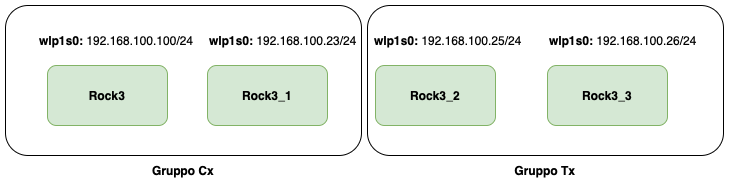
\includegraphics[width=1\textwidth]{diagramma_test.png}
    \caption{Diagramma dispositivi Rock}
    \label{fig:diagramma}
\end{figure}

Sono previsti tre principali casi di test:

\begin{itemize}
    \item \textit{T1\_C0}: assenza di QoS nei flussi dei dispositivi del \textit{Gruppo Tx} e assenza di congestione del canale, quindi il \textit{Gruppo Cx} sarà spento.
    \item \textit{T1\_C1}: assenza di QoS nei flussi dei dispositivi del \textit{Gruppo Tx} e parziale congestione del canale, attuata mediante l'invio in broadcast di CAM da ognuno dei due dispositivi facenti parte del \textit{Gruppo Cx} ogni 5 ms.
    \item \textit{T1\_C2}: assenza di QoS nei flussi dei dispositivi del \textit{Gruppo Tx} e totale congestione del canale, attuata mediante trasmissione UDP in \textit{flooding} in broadcast da parte di ognuno dei due dispositivi del \textit{Gruppo Cx}.
\end{itemize}

Questi stessi casi verranno, inoltre, ripetuti andando ad applicare delle politiche di QoS: un flusso verrà assegnato alla categoria con priorità maggiore, ovvero \textit{Access Category Voice} (AC\_VO), mentre l'altro alla categoria minore, ovvero \textit{Access Category Background} (AC\_BK).

Per fare ciò, viene utilizzato il comando iPerf, già precedentemente discusso, con i dovuti parametri. Nella fattispecie:

\begin{itemize}
    \item \textit{Rock Server}: \verb|iperf -s -i 1 -w 416K -y C -o output.csv|.
    \item \textit{Rock Client - flusso 1}: \\\verb|iperf -c 192.168.100.xxx -t 30 -b 10m -A VO| per il flusso a priorità maggiore.
    \item \textit{Rock Client - flusso 2}: \\\verb|iperf -c 192.168.100.xxx -t 30 -b 10m -A BK| per il flusso a priorità minore.
\end{itemize}

L'indirizzo IP usato nei due comandi è relativo a quello appartenente all'interfaccia \textit{wlp1s0} del dispositivo facente funzione di server.

Nei casi senza politiche di QoS sono stati utilizzati i medesimi comandi, senza ovviamente i parametri che delineano le varie priorità.

Per quanto concerne il raggiungimento di un eventuale congestione del canale, essa è stata raggiunta nei seguenti modi:

\begin{itemize}
    \item \textit{Caso senza congestione}: i dispositivi appartenenti al \textit{Gruppo Cx} non trasmettono alcunchè.
    \item \textit{Caso con congestione parziale}: i dispositivi appartenenti al \textit{Gruppo Cx}, come già detto poc'anzi, trasmettono ognuno un singolo pacchetto CAM ogni 5 ms; per tale scopo è stato lanciato sia su uno che sull'altro Rock lo script riportato in \autoref{udp_packets} con, come parametri, un \textit{message\_size} pari a 256 byte e lo \textit{sleep\_time} pari a 0.005; è stata scelto questo intervallo di tempo in quanto, tenendo conto che in caso di veicolo fermo esso invierebbe un CAM ogni 1 secondo, viene simulato un ambiente con 200 veicoli presenti.
    \item \textit{Caso con congestione totale}: i dispositivi appartenenti al \textit{Gruppo Cx} fanno flooding UDP mediante l'esecuzione del comando \verb|iperf -u -c 192.168.100.xxx| \verb| -t 300 -b 10m|; in questo caso si vuole simulare un ambiente con un numero veramente elevato di veicoli e molto maggiore del caso precedente.
\end{itemize}

In quest'ultimo caso, a causa delle limitazioni architetturali di iPerf, non è stato possibile inviare pacchetti UDP in broadcast. Poiché solo due dispositivi sono incaricati di effettuare flooding, la congestione viene raggiunta trasmettendo messaggi UDP da un dispositivo del \textit{Gruppo Cx} all'altro, specificando come parametro per iPerf l'indirizzo IP dell'interfaccia \textit{wlp1so} del Rock destinatario.

La scelta del protocollo UDP per effettuare \textit{flooding}, anzichè il TCP, è stata effettuata per ovvie ragioni: mancanza di politiche riguardanti il controllo di flusso, perdita dei pacchetti e controllo sull'ordine di ricezione di quest'ultimi. Inoltre, l'invio di essi con una dimensione inferiore a 2346 byte (iPerf, di default, invia pacchetti UDP di soli 1470 byte a differenza del TCP che hanno una dimensione pari a 8 KB \cite{iperf}), consente alle interfacce Wireless di poter trasmettere i vari frame senza attuare il meccanismo di RTS/CTS.

In conclusione, per ogni simulazione sono state effettuati 5 \textit{run} distinti, ciascuno della durata di 30 secondi. Questa scelta è stata fatta per ottenere risultati il più affidabili possibile, escludendo la parte iniziale dell'handshake del protocollo TCP, che potrebbe influenzare i valori iniziali in modo non desiderato.

Verranno, ora, mostrati i risultati ottenuti mediante dei grafici per ogni singolo caso di studio:

\begin{itemize}
    \item il primo mostrerà l'andamento del throughput medio nel corso della simulazione;
    \item il secondo consisterà nel \textit{plot} del throughput di ogni singola \textit{run};
    \item il terzo visualizzerà il carico del canale per tutta la durata della simulazione, inclusi alcuni istanti primae e dopo in modo da mostrare le condizioni iniziali.
\end{itemize}

\noindent I grafici sono stati generati mediante codice \textit{Python} usando la libreria \textit{matplotlib}; i codici sorgenti possono essere trovati nella \autoref{plot_test1}, \autoref{plot_test_spaghetti} e \autoref{plot_test_load}.

Alla fine verranno fatte le dovute considerazioni del caso.

\subsection[QoS assente e congestione assente]{QoS assente e congestione assente}
L'assenza di politiche di QoS, unito ad un canale quasi completamente vuoto e libero da trasmissioni (Figura \ref{fig:t1_c0_load}), porta il throughput di ambedue i flussi ad essere simile al netto di una differenza trascurabile (Tabella \ref{table:6}). Sul canale è possibile trasmettere sino ad un massimo di 10 Mbps teorici, quindi si può tranquillamente notare che le due trasmissioni si suddividono equamente la banda disponibile (Figure \ref{fig:t1_c0} e \ref{fig:t1_c0_ensemble}).

\begin{table}[h!]
    \centering
    \begin{tabular}{|>{\centering\arraybackslash}p{20em}|>{\centering\arraybackslash}p{7em}|} 
     \hline
     \textbf{} & \textbf{Valori} \\ 
     \hline
     \textbf{Throughput Medio per Stream ID 1} & 3.49 Mbps \\ 
     \hline
     \textbf{Throughput Medio per Stream ID 2} & 3.47 Mbps \\
     \hline
    \end{tabular}
    \caption{Valori medi caso QoS assente e congestione assente}
    \label{table:6}
\end{table}

\begin{figure}[h!]
    \centering
    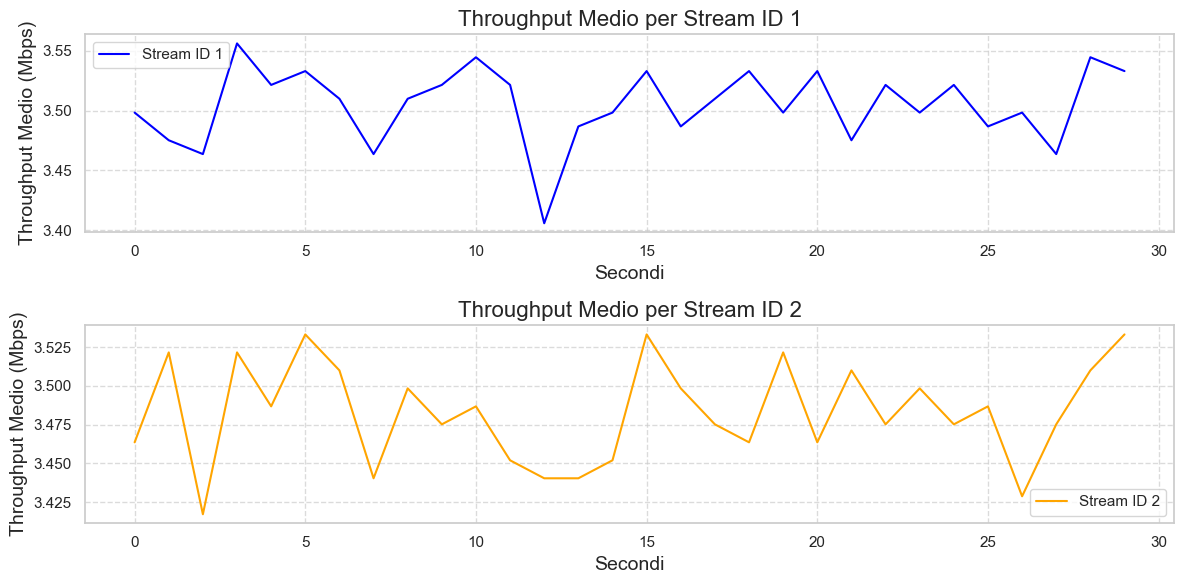
\includegraphics[width=1\textwidth]{t1_c0.png}
    \caption{QoS assente e congestione assente (Throughput medio)}
    \label{fig:t1_c0}
\end{figure}

\begin{figure}[h!]
    \centering
    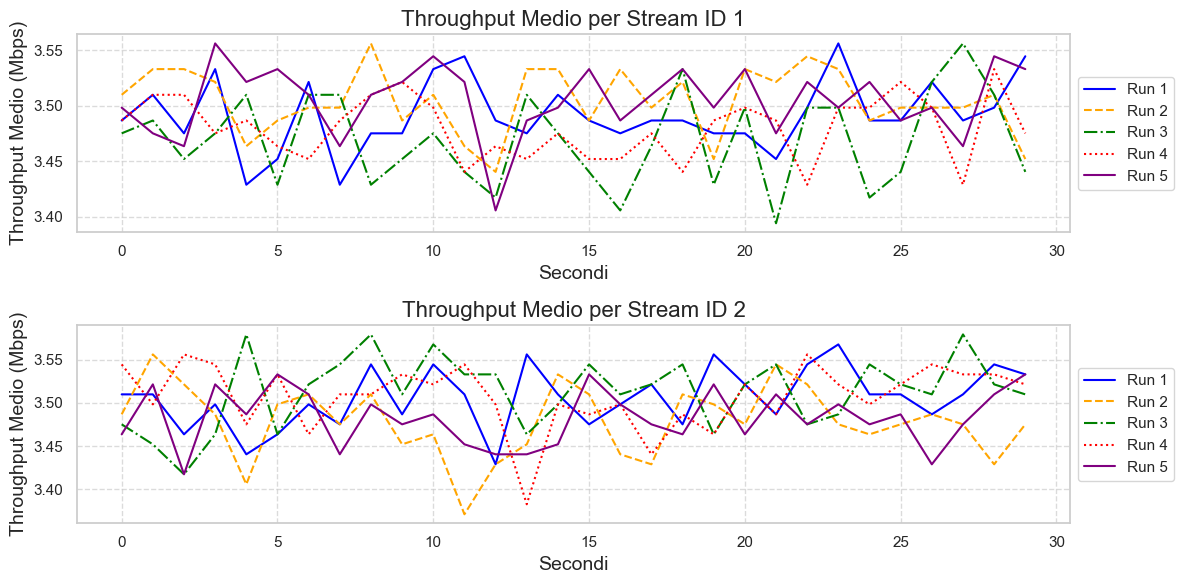
\includegraphics[width=1\textwidth]{t1_c0_ensemble.png}
    \caption{QoS assente e congestione assente (Grafico ensemble)}
    \label{fig:t1_c0_ensemble}
\end{figure}
\clearpage
\begin{figure}[h!]
    \centering
    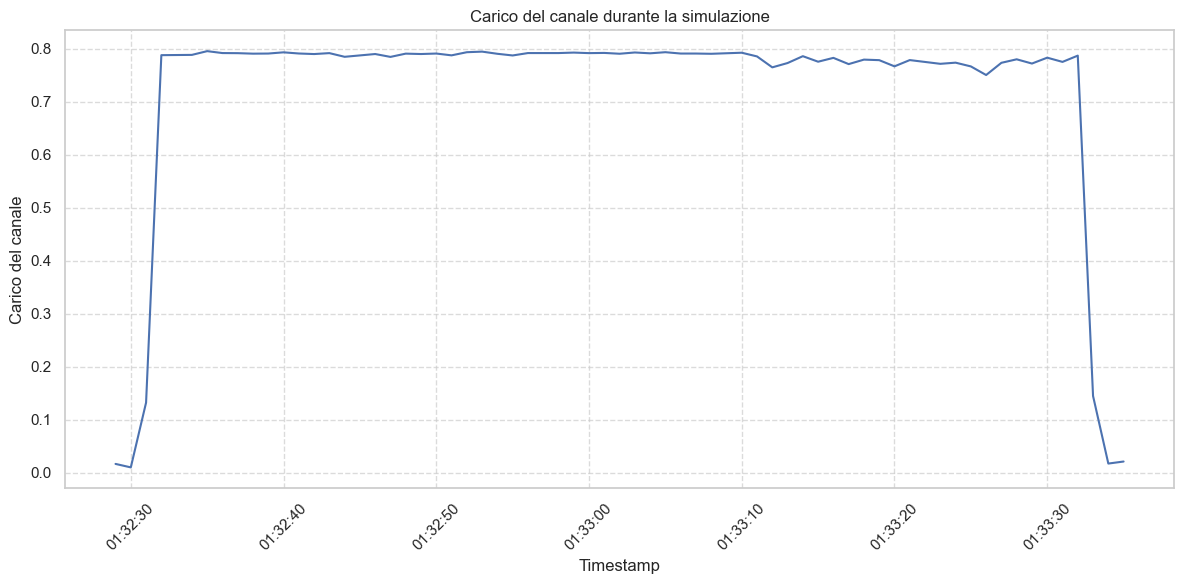
\includegraphics[width=1\textwidth]{t1_c0_load.png}
    \caption{QoS assente e congestione assente (Carico del canale)}
    \label{fig:t1_c0_load}
\end{figure}

\subsection[QoS assente e congestione parziale]{QoS assente e congestione parziale}
L'assenza di politiche di QoS, unito ad un canale parzialmente disturbato da CAM inviati dagli altri due dispositivi (Figura \ref{fig:t1_c1_load}), porta il throughput di ambedue i flussi ad essere simile ma inferiore rispetto al caso precedentemente discusso di circa il 10\%: 3.49 Mbps circa contro 3.13 Mbps qui (Tabella \ref{table:7} e Figure \ref{fig:t1_c1} e \ref{fig:t1_c1_ensemble}).

\begin{table}[h!]
    \centering
    \begin{tabular}{|>{\centering\arraybackslash}p{20em}|>{\centering\arraybackslash}p{7em}|} 
     \hline
     \textbf{} & \textbf{Valori} \\ 
     \hline
     \textbf{Throughput Medio per Stream ID 1} & 3.13 Mbps \\ 
     \hline
     \textbf{Throughput Medio per Stream ID 2} & 3.13 Mbps \\
     \hline
    \end{tabular}
    \caption{Valori medi caso QoS assente e congestione parziale}
    \label{table:7}
\end{table}

\begin{figure}[h!]
    \centering
    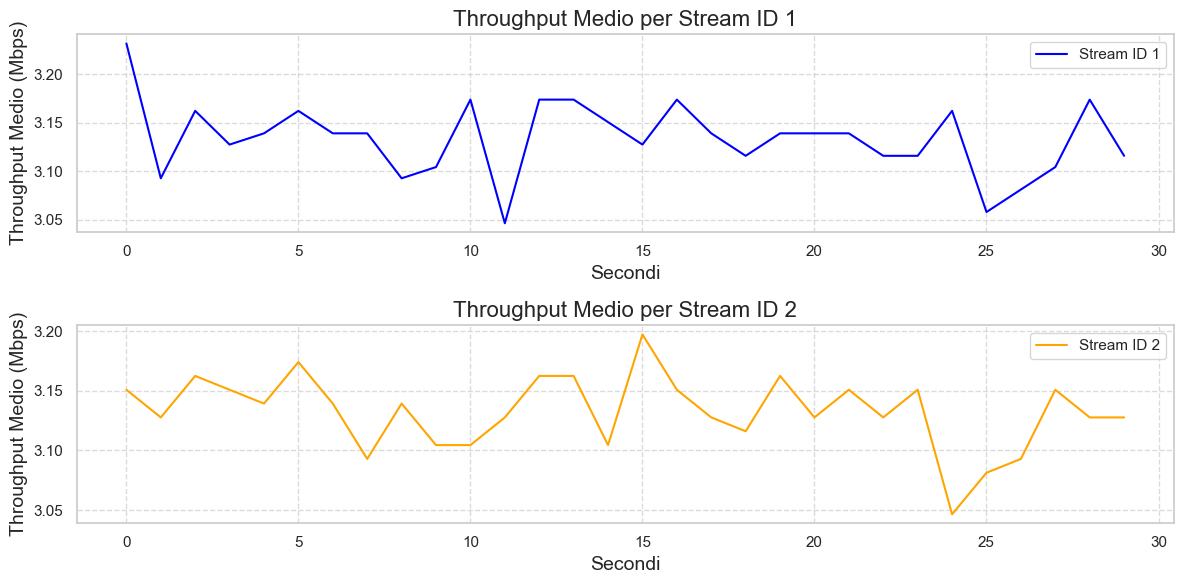
\includegraphics[width=1\textwidth]{t1_c1.png}
    \caption{QoS assente e congestione parziale (Throughput medio)}
    \label{fig:t1_c1}
\end{figure}

\begin{figure}[h!]
    \centering
    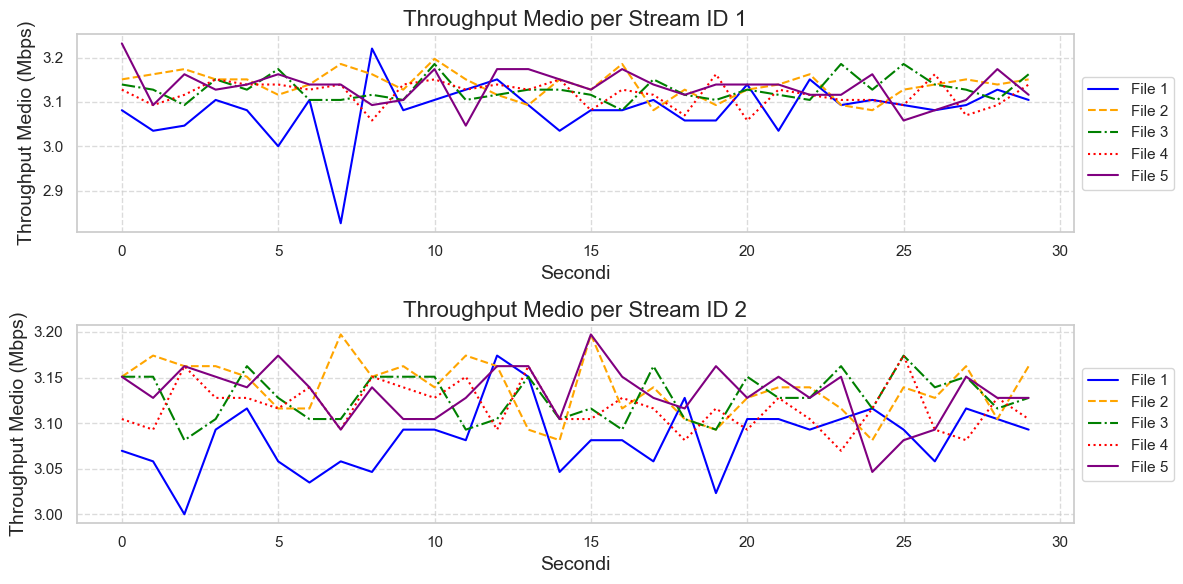
\includegraphics[width=1\textwidth]{t1_c1_ensemble.png}
    \caption{QoS assente e congestione parziale (Grafico ensemble)}
    \label{fig:t1_c1_ensemble}
\end{figure}
\clearpage
\begin{figure}[h!]
    \centering
    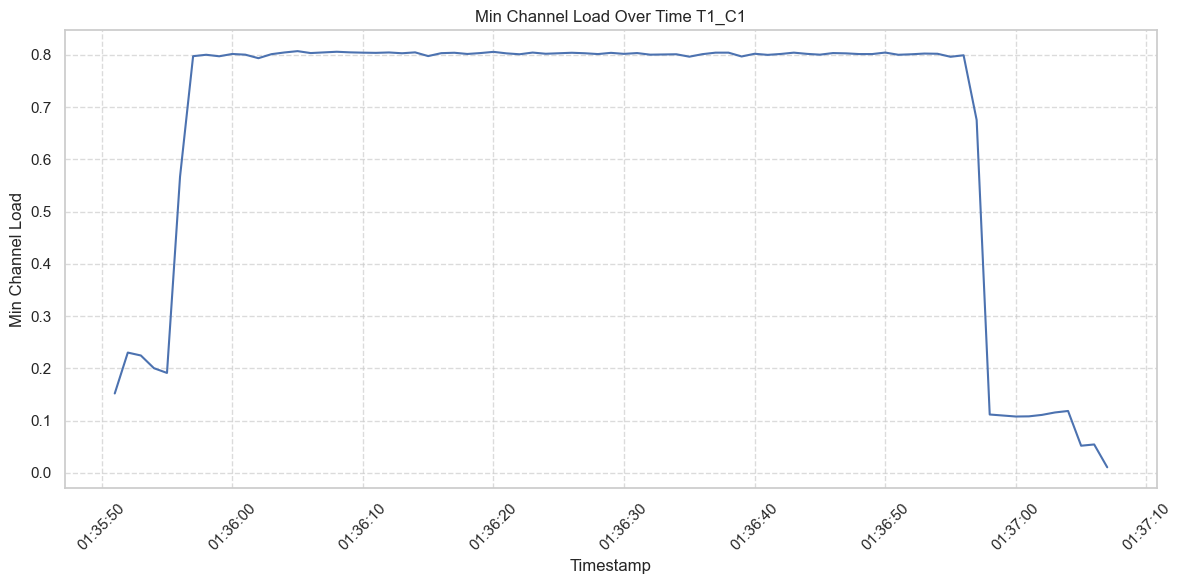
\includegraphics[width=1\textwidth]{t1_c1_load.png}
    \caption{QoS assente e congestione parziale (Carico del canale)}
    \label{fig:t1_c1_load}
\end{figure}

\subsection[QoS assente e congestione totale]{QoS assente e congestione totale}
La completa saturazione del canale qui si fa sentire notevolmente (Figura \ref{fig:t1_c2_load}), in quanto il throughput di ambedue i flussi viene ridotto notevolmente con una minore propensione ad essere stabile rispetto al caso senza congestione: 3.49 Mbps circa contro 1.14 Mbps circa qui (Tabella \ref{table:8} e Figure \ref{fig:t1_c2} e \ref{fig:t1_c2_ensemble}).
\begin{table}[h!]
    \centering
    \begin{tabular}{|>{\centering\arraybackslash}p{20em}|>{\centering\arraybackslash}p{7em}|} 
     \hline
     \textbf{} & \textbf{Valori} \\ 
     \hline
     \textbf{Throughput Medio per Stream ID 1} & 1.14 Mbps \\ 
     \hline
     \textbf{Throughput Medio per Stream ID 2} & 1.19 Mbps \\
     \hline
    \end{tabular}
    \caption{Valori medi caso QoS assente e congestione totale}
    \label{table:8}
\end{table}

\begin{figure}[h!]
    \centering
    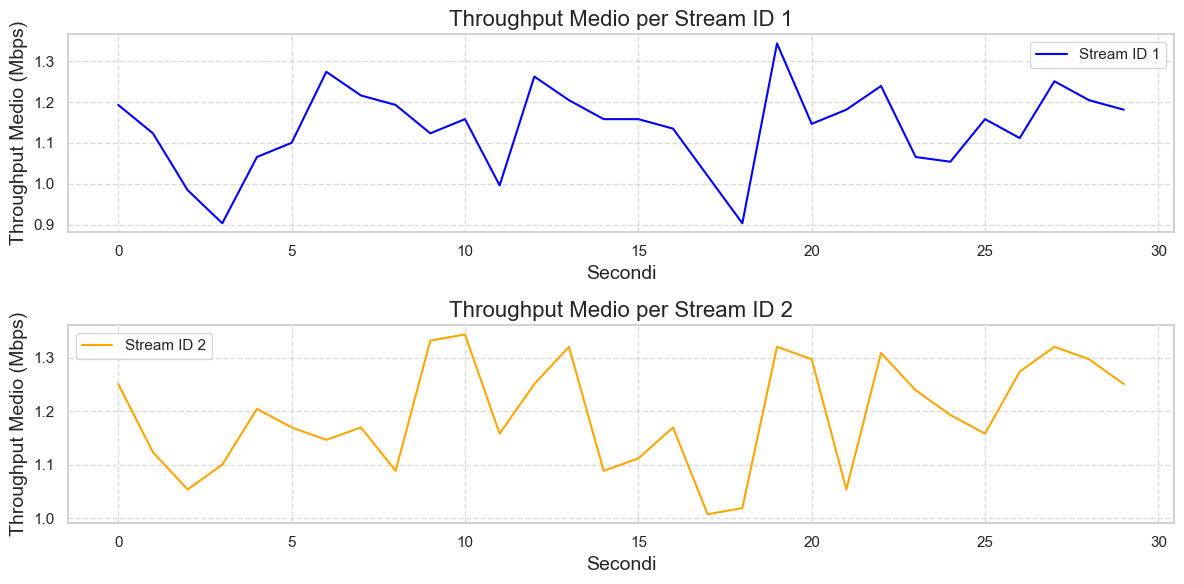
\includegraphics[width=1\textwidth]{t1_c2.png}
    \caption{QoS assente e congestione totale (Throughput medio)}
    \label{fig:t1_c2}
\end{figure}

\begin{figure}[h!]
    \centering
    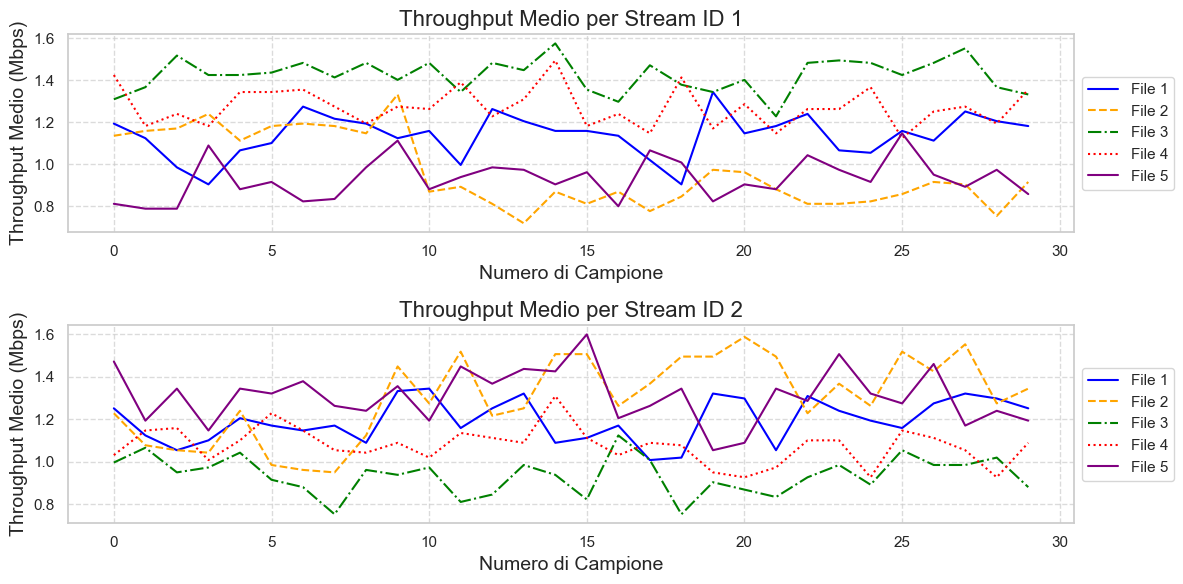
\includegraphics[width=1\textwidth]{t1_c2_ensemble.png}
    \caption{QoS assente e congestione totale (Grafico ensemble)}
    \label{fig:t1_c2_ensemble}
\end{figure}
\clearpage
\begin{figure}[h!]
    \centering
    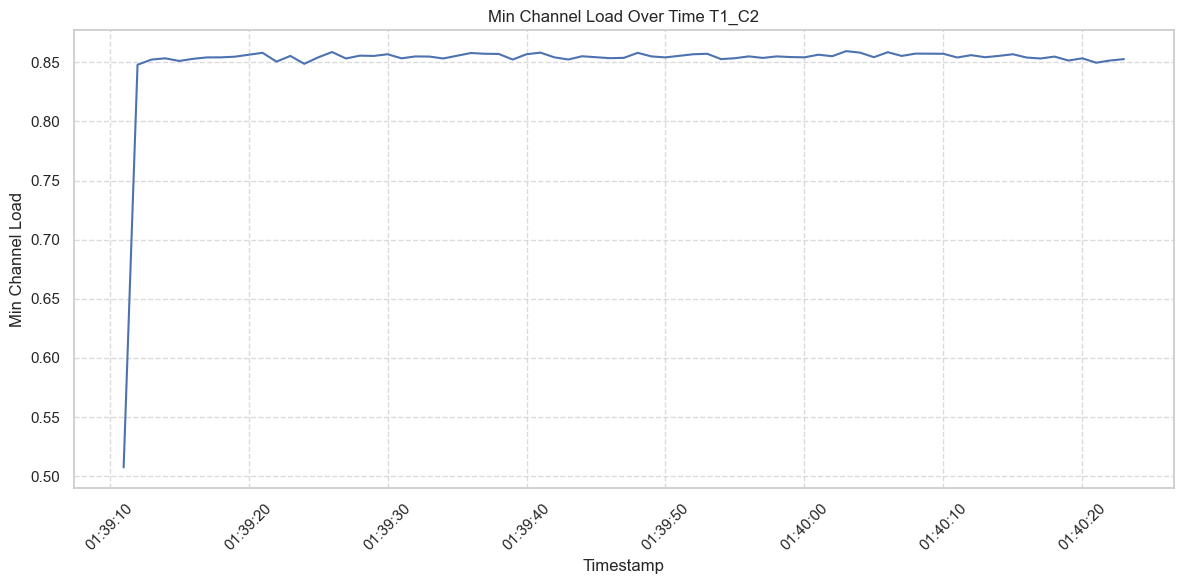
\includegraphics[width=1\textwidth]{t1_c2_load.png}
    \caption{QoS assente e congestione totale (Carico del canale)}
    \label{fig:t1_c2_load}
\end{figure}

\subsection[QoS presente e congestione assente]{QoS presente e congestione assente}
L'inserimento, qui, di politiche di QoS, unito ad un canale quasi completamente vuoto e libero da trasmissioni (Figura \ref{fig:t2_c0_load}), porta il throughput del flusso a priorità maggiore ad sorpaffare completamente l'altro a priorità minore (Tabella \ref{table:9} e Figure \ref{fig:t2_c0} e \ref{fig:t2_c0_ensemble}).

\begin{table}[h!]
    \centering
    \begin{tabular}{|>{\centering\arraybackslash}p{20em}|>{\centering\arraybackslash}p{7em}|} 
     \hline
     \textbf{} & \textbf{Valori} \\ 
     \hline
     \textbf{Throughput Medio per Stream ID 1} & 7.96 Mbps \\ 
     \hline
     \textbf{Throughput Medio per Stream ID 2} & 0.61 Mbps \\
     \hline
    \end{tabular}
    \caption{Valori medi caso QoS presente e congestione assente}
    \label{table:9}
\end{table}

\begin{figure}[h!]
    \centering
    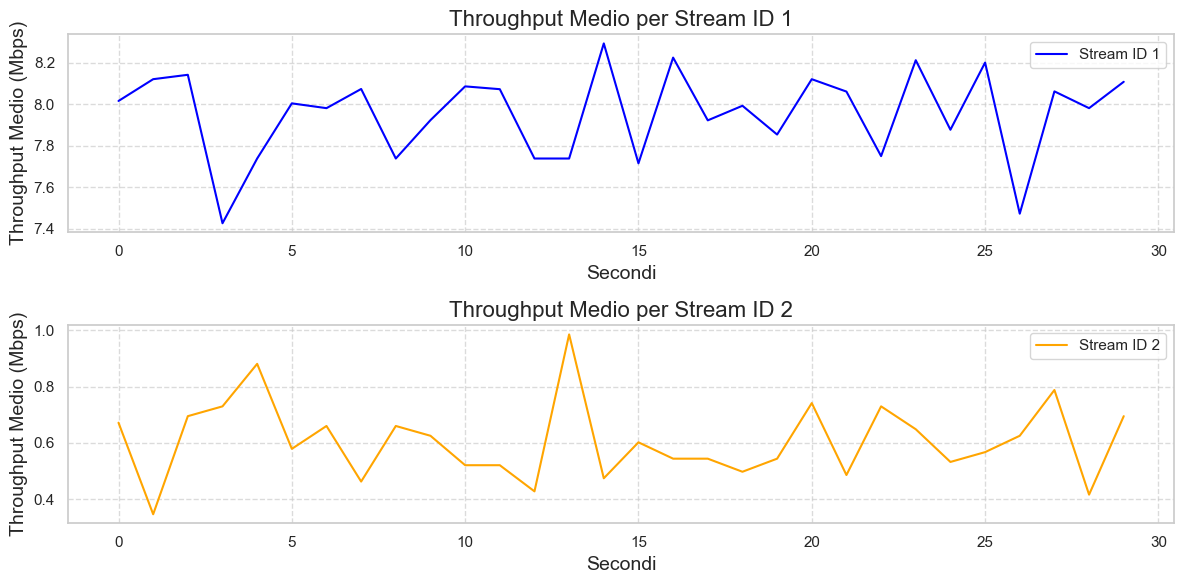
\includegraphics[width=1\textwidth]{t2_c0.png}
    \caption{QoS presente e congestione assente (Throughput medio)}
    \label{fig:t2_c0}
\end{figure}

\begin{figure}[h!]
    \centering
    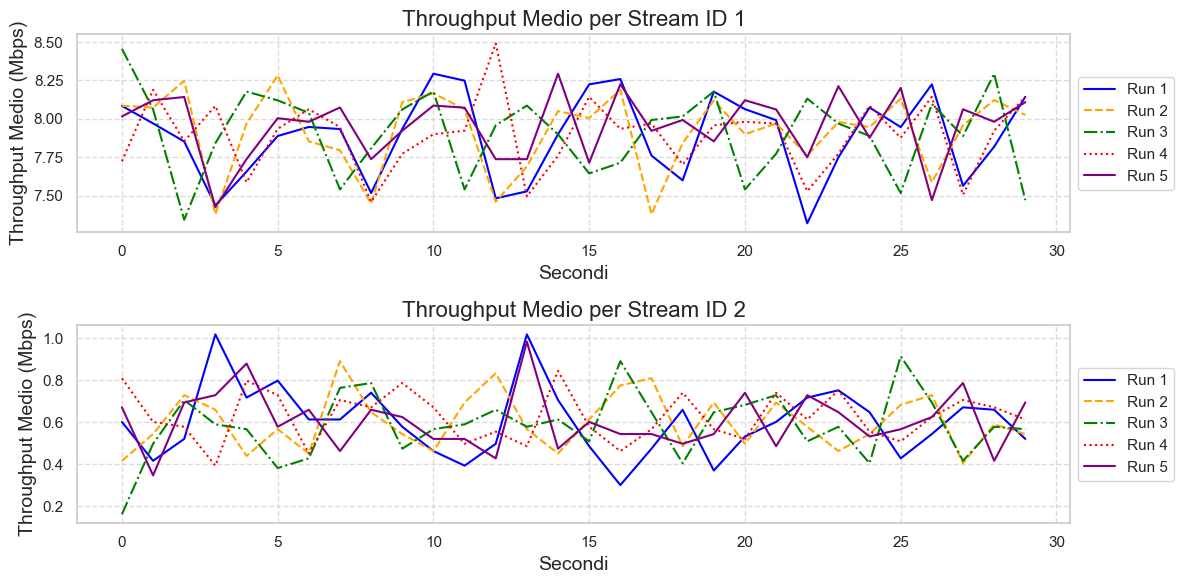
\includegraphics[width=1\textwidth]{t2_c0_ensemble.png}
    \caption{QoS presente e congestione assente (Grafico ensemble)}
    \label{fig:t2_c0_ensemble}
\end{figure}
\clearpage
\begin{figure}[h!]
    \centering
    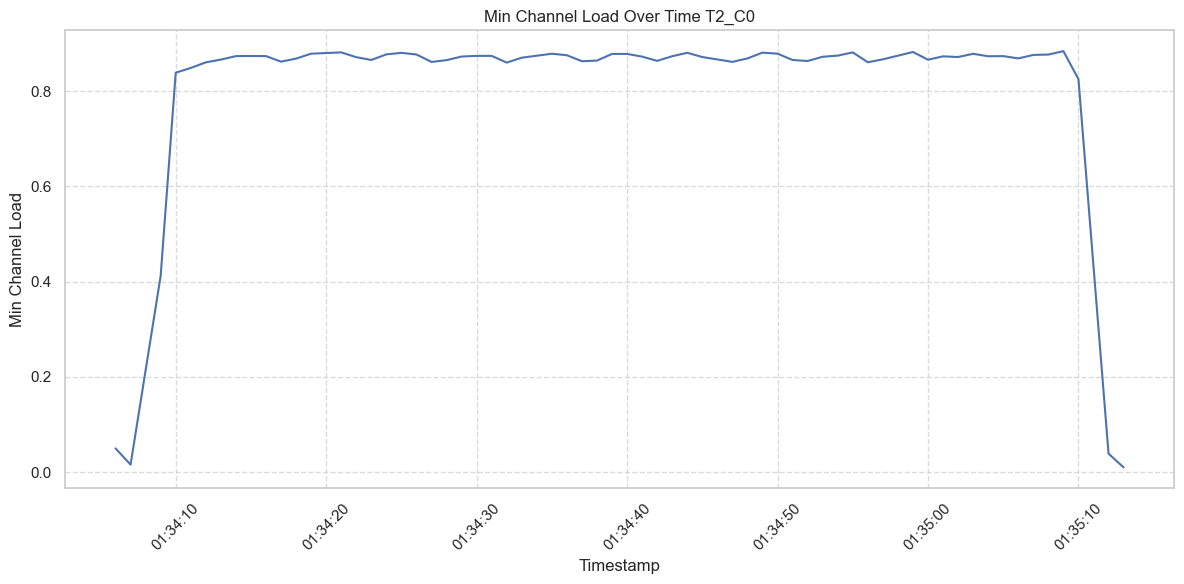
\includegraphics[width=1\textwidth]{t2_c0_load.png}
    \caption{QoS presente e congestione assente (Carico del canale)}
    \label{fig:t2_c0_load}
\end{figure}

\subsection[QoS presente e congestione parziale]{QoS presente e congestione parziale}
Che scrivo qui? XD
\begin{table}[h!]
    \centering
    \begin{tabular}{|>{\centering\arraybackslash}p{20em}|>{\centering\arraybackslash}p{7em}|} 
     \hline
     \textbf{} & \textbf{Valori} \\ 
     \hline
     \textbf{Throughput Medio per Stream ID 1} & 6.73 Mbps \\ 
     \hline
     \textbf{Throughput Medio per Stream ID 2} & 0.77 Mbps \\
     \hline
    \end{tabular}
    \caption{Valori medi caso QoS presente e congestione parziale}
    \label{table:10}
\end{table}

\begin{figure}[h!]
    \centering
    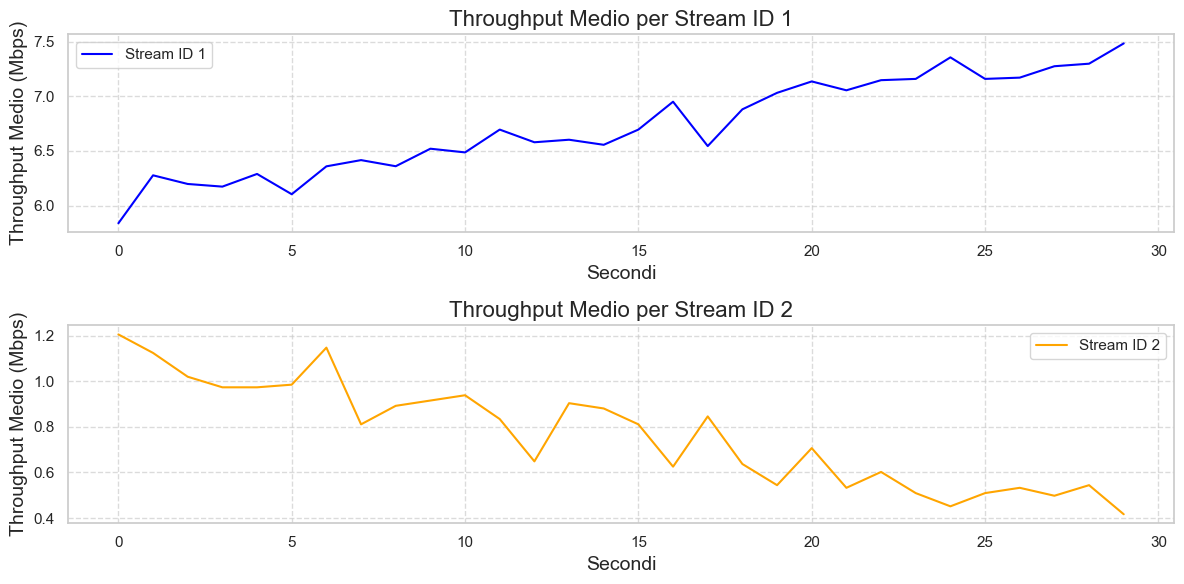
\includegraphics[width=1\textwidth]{t2_c1.png}
    \caption{QoS presente e congestione parziale (Throughput medio)}
    \label{fig:t2_c1}
\end{figure}

\begin{figure}[h!]
    \centering
    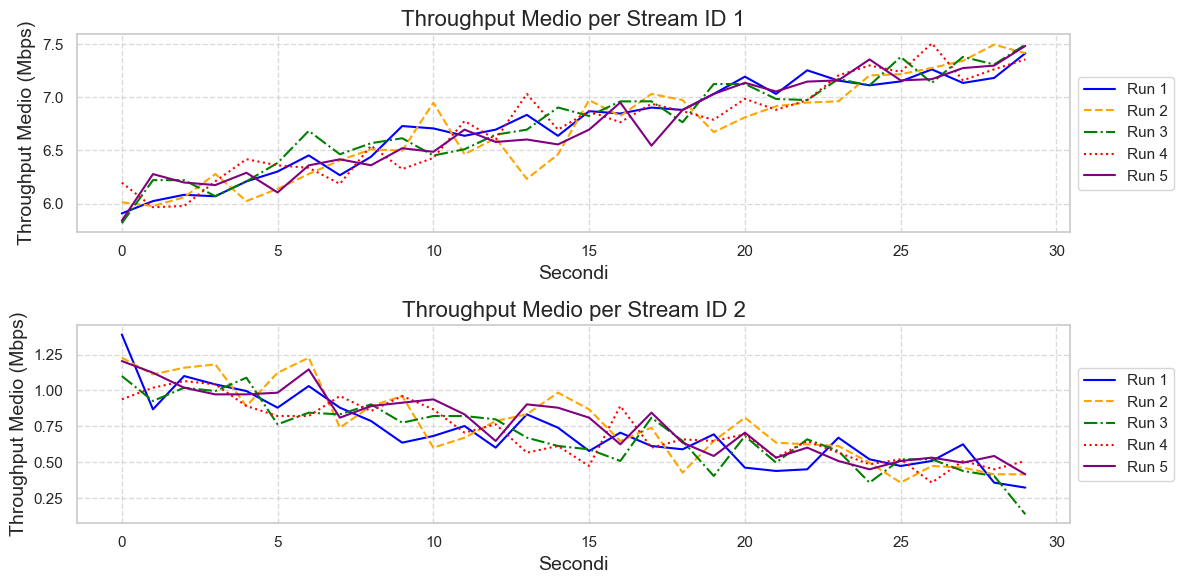
\includegraphics[width=1\textwidth]{t2_c1_ensemble.png}
    \caption{QoS presente e congestione parziale (Grafico ensemble)}
    \label{fig:t2_c1_ensemble}
\end{figure}
\clearpage
\begin{figure}[h!]
    \centering
    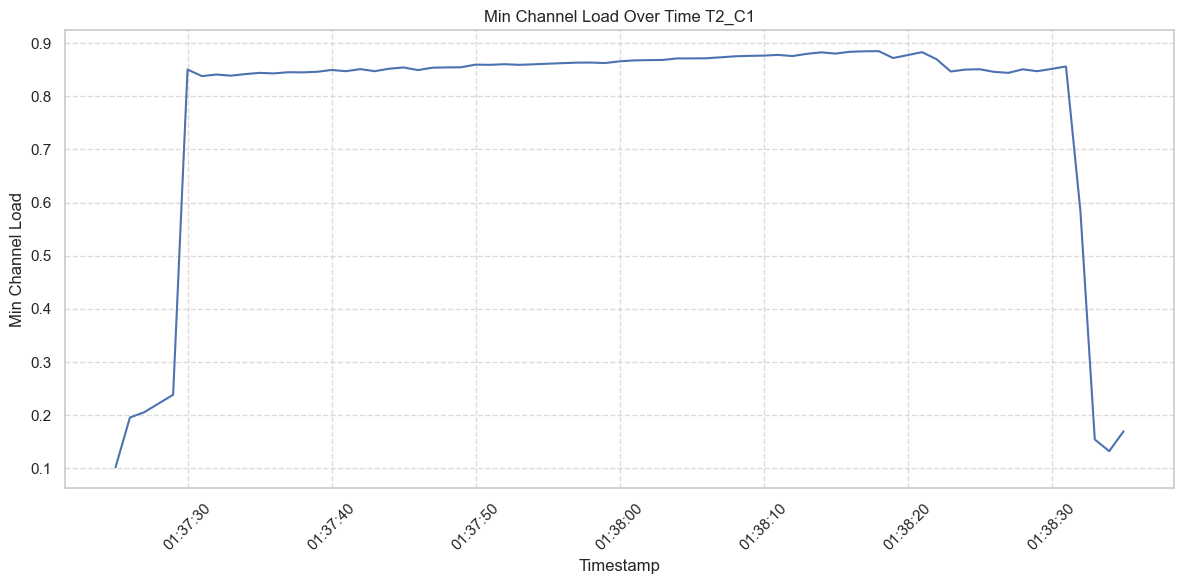
\includegraphics[width=1\textwidth]{t2_c1_load.png}
    \caption{QoS presente e congestione parziale (Carico del canale)}
    \label{fig:t2_c1_load}
\end{figure}

\subsection[QoS presente e congestione totale]{QoS presente e congestione totale}
La completa saturazione del canale qui si fa sentire notevolmente (Figura \ref{fig:t2_c2_load}), in quanto il throughput di ambedue i flussi viene ridotto notevolmente con un inoltre minore propensione ad essere stabile rispetto al caso senza congestione. (Tabella \ref{table:11} e Figure \ref{fig:t2_c2} e \ref{fig:t2_c2_ensemble}). L'applicazione di politiche di QoS porta, naturalmente, ad un throughput medio maggiore del flusso a priorità maggiore.

\begin{table}[h!]
    \centering
    \begin{tabular}{|>{\centering\arraybackslash}p{20em}|>{\centering\arraybackslash}p{7em}|} 
     \hline
     \textbf{} & \textbf{Valori} \\ 
     \hline
     \textbf{Throughput Medio per Stream ID 1} & 6.19 Mbps \\ 
     \hline
     \textbf{Throughput Medio per Stream ID 2} & 0.30 Mbps \\
     \hline
    \end{tabular}
    \caption{Valori medi caso QoS presente e congestione totale}
    \label{table:11}
\end{table}

\begin{figure}[h!]
    \centering
    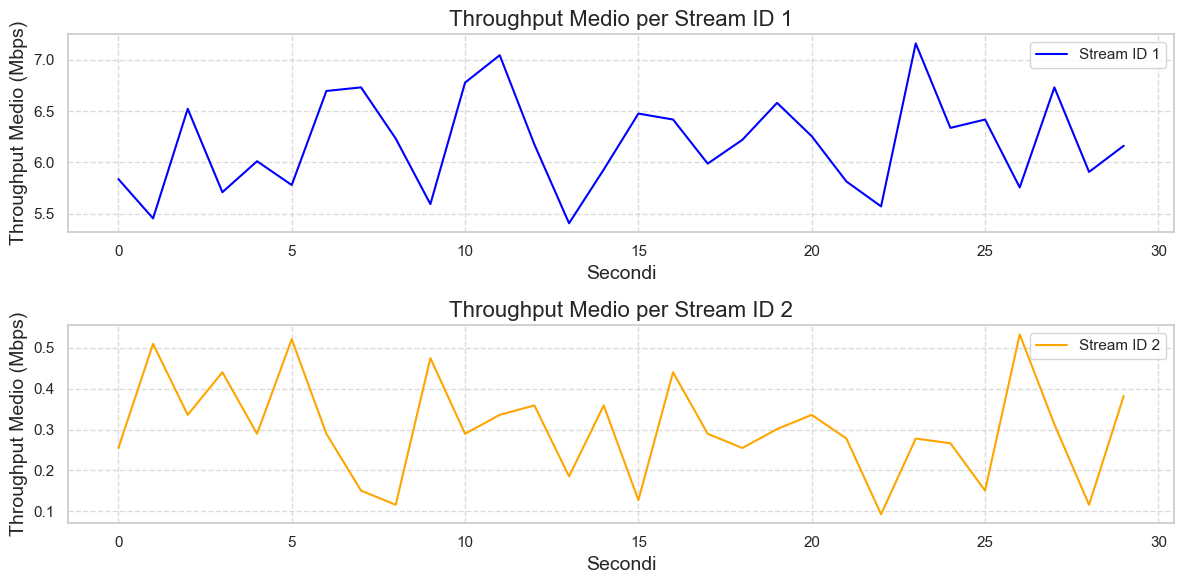
\includegraphics[width=1\textwidth]{t2_c2.png}
    \caption{QoS presente e congestione totale (Throughput medio)}
    \label{fig:t2_c2}
\end{figure}

\begin{figure}[h!]
    \centering
    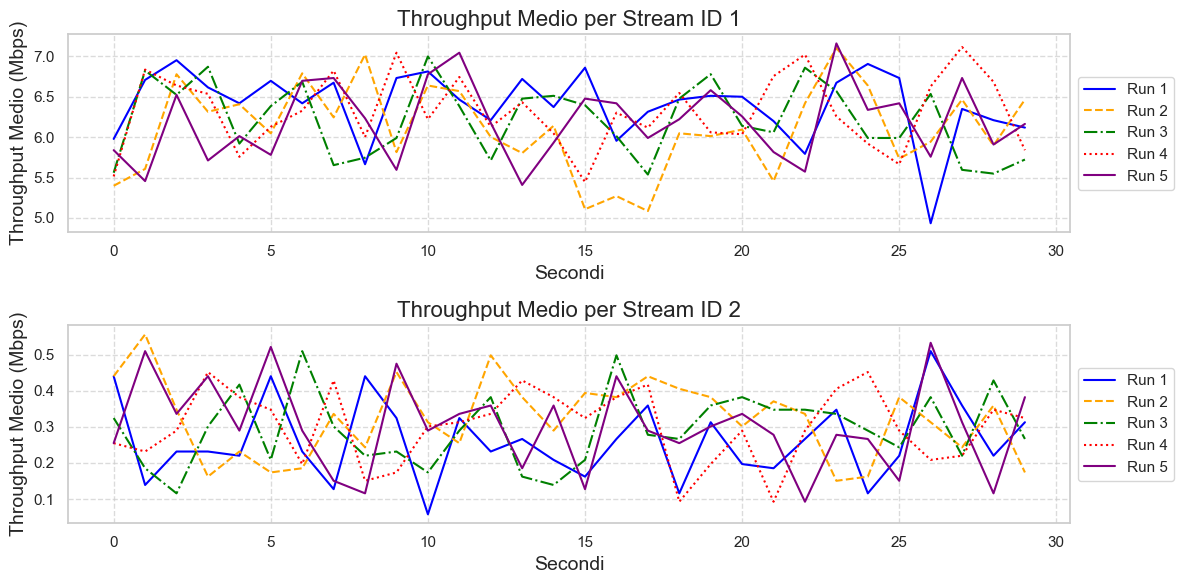
\includegraphics[width=1\textwidth]{t2_c2_ensemble.png}
    \caption{QoS presente e congestione totale (Grafico ensemble)}
    \label{fig:t2_c2_ensemble}
\end{figure}
\clearpage
\begin{figure}[h!]
    \centering
    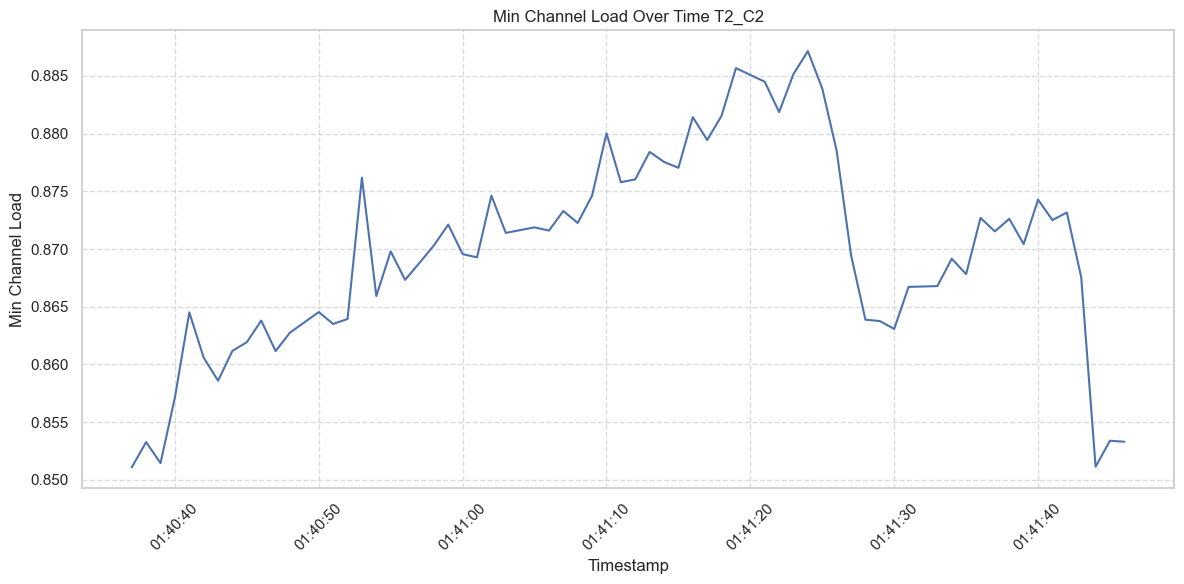
\includegraphics[width=1\textwidth]{t2_c2_load.png}
    \caption{QoS presente e congestione totale (Carico del canale)}
    \label{fig:t2_c2_load}
\end{figure}
\subsection[Analisi dei risultati]{Analisi dei risultati}
Da come è stato possibile notare dai dati raccolti e mostrati nelle sottosezioni precendenti (Tabella \ref{table:12}), la presenza di disturbi più o meno marcati influenza, anche solo parzialmente, la trasmissione dei due flussi TCP dal nodo server al nodo client.

Si passa da throughput elevato e relativamente stabile, a prestazioni man mano più basse, evidenziando anche una tendenza della velocità media ad essere meno stabile e più suscettibile di oscillazioni.

Questo discorso è applicabile sia nei casi in cui non sono state implementate politiche di QoS, sia quando si assegna una maggiore priorità a uno dei flussi rispetto all'altro. Anche in queste situazioni, si osservano valori di throughput medio generalmente meno stabili e caratterizzati da oscillazioni nel tempo; in effetti, la variabilità tende a peggiorare in tutti i casi di congestione.

Pertanto, si può concludere che l'uso di diverse Access Categories non ha effetti positivi sulla variabilità del throughput, che continua a oscillare in presenza di congestione. L'unico effetto riscontrato è la maggiore velocità del flusso con priorità maggiore a discapito di quello a priorità minore.
\clearpage
\begin{table}[h!]
    \centering
    \begin{tabular}{|p{20em}|>{\centering\arraybackslash}p{5em}|>{\centering\arraybackslash}p{5em}|} 
     \hline
     \textbf{Caso} & \textbf{Valori} & \textbf{Varianza}\\ 
     \hline
     \textbf{QoS assente e congestione assente (Stream 1)} & 3.49 & 0.000972\\ 
     \hline
     \textbf{QoS assente e congestione assente (Stream 2)} & 3.47 & 0.000972 \\
     \hline
     \textbf{QoS assente e congestione parziale (Stream 1)} & 3.13 & 0.00144\\ 
     \hline
     \textbf{QoS assente e congestione parziale (Stream 2)} & 3.13 & 0.00092\\
     \hline
     \textbf{QoS assente e congestione totale (Stream 1)} & 1.14 & 0.0919\\ 
     \hline
     \textbf{QoS assente e congestione totale (Stream 2)} & 1.19 & 0.01540\\
     \hline
     \textbf{QoS presente e congestione assente (Stream 1)} & 7.96 & 0.04425\\ 
     \hline
     \textbf{QoS presente e congestione assente (Stream 2)} & 0.61 & 0.01867\\
     \hline
     \textbf{QoS presente e congestione parziale (Stream 1)} & 6.73 & 0.1835\\ 
     \hline
     \textbf{QoS presente e congestione parziale (Stream 2)} & 0.77 & 0.04963\\
     \hline
     \textbf{QoS presente e congestione totale (Stream 1)} & 6.19 & 0.20920\\ 
     \hline
     \textbf{QoS presente e congestione totale (Stream 2)} & 0.30 & 0.01466\\
     \hline
    \end{tabular}
    \caption{Confronti risultati (Valori in Mbps)}
    \label{table:12}
\end{table}
\section{Test 2}

\section{Lost packets}

\chapter{Conclusion}

\section{Hello World}
Ciao

\chapter{Appendice}

\section{Patch iPerf per AC}
\label{iperf_ac}
\begin{lstlisting}
    --- a/include/Settings.hpp
    +++ b/include/Settings.hpp
    @@ -135,6 +135,7 @@ typedef struct thread_Settings {
         // int's
         int mThreads;                   // -P
         int mTOS;                       // -S
    +    int mMACUP;                     // -A
     #if WIN32
         SOCKET mSock;
     #else
    --- a/include/version.h
    +++ b/include/version.h
    @@ -1,4 +1,4 @@
    -#define IPERF_VERSION "2.0.13"
    +#define IPERF_VERSION "2.0.13 OpenWrt-V2X patch"
     #define IPERF_VERSION_DATE "21 Jan 2019"
     #define IPERF_VERSION_MAJORHEX 0x00020000
     #define IPERF_VERSION_MINORHEX 0x000D0003
    --- a/src/Locale.c
    +++ b/src/Locale.c
    @@ -103,6 +103,7 @@ Server specific:\n\
       -s, --server             run in server mode\n\
       -t, --time      #        time in seconds to listen for new connections as well as to receive traffic (default not set)\n\
           --udp-histogram #,#  enable UDP latency histogram(s) with bin width and count, e.g. 1,1000=1(ms),1000(bins)\n\
    +  -A, --accesscategory <AC> Forces a certain EDCA MAC access category to be used (BK, BE, VI, VO)\n\
       -B, --bind <ip>[%<dev>]  bind to multicast address and optional device\n\
       -H, --ssm-host <ip>      set the SSM source, use with -B for (S,G) \n\
       -U, --single_udp         run in single threaded UDP mode\n\
    @@ -125,6 +126,7 @@ Client specific:\n\
     "  -n, --num       #[kmgKMG]    number of bytes to transmit (instead of -t)\n\
       -r, --tradeoff           Do a bidirectional test individually\n\
       -t, --time      #        time in seconds to transmit for (default 10 secs)\n\
    +  -A, --accesscategory <AC> Forces a certain EDCA MAC access category to be used (BK, BE, VI, VO)\n\
       -B, --bind [<ip> | <ip:port>] bind ip (and optional port) from which to source traffic\n\
       -F, --fileinput <name>   input the data to be transmitted from a file\n\
       -I, --stdin              input the data to be transmitted from stdin\n\
    --- a/src/PerfSocket.cpp
    +++ b/src/PerfSocket.cpp
    @@ -155,6 +155,15 @@ void SetSocketOptions( thread_Settings *
         }
     #endif
     
    +   	// set MAC AC (access category) field, if specified only (i.e. if mMACUP != -1)
    +    // AC is set starting from user priorities (UP)
    +	if ( inSettings->mMACUP >= 0 ) {
    +		int  up = inSettings->mMACUP;
    +		Socklen_t len = sizeof(up);
    +		int rc = setsockopt( inSettings->mSock, SOL_SOCKET, SO_PRIORITY, (char*) &up, len );
    +		WARN_errno( rc == SOCKET_ERROR, "setsockopt SO_PRIORITY" );
    +	}
    +
         if ( !isUDP( inSettings ) ) {
             // set the TCP maximum segment size
             setsock_tcp_mss( inSettings->mSock, inSettings->mMSS );
    --- a/src/Settings.cpp
    +++ b/src/Settings.cpp
    @@ -131,6 +131,7 @@ const struct option long_options[] =
     {"realtime",         no_argument, NULL, 'z'},
     
     // more esoteric options
    +{"accesscategory",  required_argument, NULL, 'A'},
     {"bind",       required_argument, NULL, 'B'},
     {"compatibility",    no_argument, NULL, 'C'},
     {"daemon",           no_argument, NULL, 'D'},
    @@ -198,6 +199,7 @@ const struct option env_options[] =
     {"IPERF_REPORTSTYLE",required_argument, NULL, 'y'},
     
     // more esoteric options
    +{"IPERF_MACAC",        required_argument, NULL, 'A'},
     {"IPERF_BIND",       required_argument, NULL, 'B'},
     {"IPERF_COMPAT",           no_argument, NULL, 'C'},
     {"IPERF_DAEMON",           no_argument, NULL, 'D'},
    @@ -218,7 +220,8 @@ const struct option env_options[] =
     
     #define SHORT_OPTIONS()
     
    -const char short_options[] = "1b:c:def:hi:l:mn:o:p:rst:uvw:x:y:zB:CDF:H:IL:M:NP:RS:T:UVWXZ:";
    +// Edited to add the A: (A + 1 argument) short option
    +const char short_options[] = "1b:c:def:hi:l:mn:o:p:rst:uvw:x:y:zA:B:CDF:IL:M:NP:RS:T:UVWZ:";
     
     /* ------------------------------------------------------
      * defaults
    @@ -279,6 +282,7 @@ void Settings_Initialize( thread_Setting
         //main->mThreads      = 0;           // -P,
         //main->mRemoveService = false;      // -R,
         //main->mTOS          = 0;           // -S,  ie. don't set type of service
    +    main->mMACUP        = -1;            // -A (set to an invalid number as default -> with -1 no setsockopt will be called for AC)
         main->mTTL          = -1;            // -T,  link-local TTL
         //main->mDomain     = kMode_IPv4;    // -V,
         //main->mSuggestWin = false;         // -W,  Suggest the window size.
    @@ -692,6 +696,24 @@ void Settings_Interpret( char option, co
                 mExtSettings->mTOS = strtol( optarg, NULL, 0 );
                 break;
     
    +        case 'A': // 802.11p/802.11e MAC layer access categories
    +            // Mapping between UP (0 to 7) and AC (BK to VO)
    +            if(strcmp(optarg,"BK") == 0) {
    +                mExtSettings->mMACUP=1; // UP=1 (2) is AC_BK
    +            } else if(strcmp(optarg,"BE") == 0) {
    +                mExtSettings->mMACUP=0; // UP=0 (3) is AC_BE
    +            } else if(strcmp(optarg,"VI") == 0) {
    +                mExtSettings->mMACUP=4; // UP=4 (5) is AC_VI
    +            } else if(strcmp(optarg,"VO") == 0) {
    +                mExtSettings->mMACUP=6; // UP=6 (7) is AC_VO
    +            } else {
    +                // Leave to default (-1), i.e. no AC is set to socket, and print error
    +                fprintf(stderr, "Invalid AC specified with -A\nValid ones are: BK, BE, VI, VO\nNo AC will be set\n");
    +            }
    +
    +            //mExtSettings->mMACUP = strtol( optarg, NULL, 0 );
    +            break;
    +
             case 'T': // time-to-live for both unicast and multicast
                 mExtSettings->mTTL = atoi( optarg );
                 break;
\end{lstlisting}

%\chapter*{Appendice}
appendix
\newpage
\bibliographystyle{unsrt} % o un altro stile bibliografico di tua scelta
\bibliography{bibliography}

\thispagestyle{plain}

\section*{Ringraziamenti}
Ringrazio mamma, papà ed Emiliano ed Antonio e Solida e Luca e Luca e Feli e Fede etc etc

\end{document}
